% ===================================================================
% Arquivo: capitulos/parte-III-pilares/cap-10-perda-binaria.tex
% ===================================================================

\chapter{Funções de Perda para Regressão}
\label{cap:perda-regressao}

Agora agora foi visto o funcionamento da retropropagação, e como ela faz uso dos otimizadores, os quais funcionam como um barco, percorendo as ondas em busca dos pontos de mínimo. Além disso, foram vistas em seguida diversas funções de ativação, começando pelas sigmoidais, depois pelas retificadoras, e por fim uma coletânea de diferentes funções. Contudo, está na hora de entender um outro lado da retropropagação: as funções de perda, as quais são justamente as ondas que os otimizadores percorrem.

Para isso, esse capítulo busca explicar algumas dos diferentes tipos de funções de perda, mais precisamente as funções de perda para tarefas de regressão. Assim, o capítulo pode ser dividido em quatro grandes partes: funções de perda para prorósitos gerais, funções de perda para medir o erro relativo, funções que vão além do cálculo da média dos erros, por último funções que são utilizadas para problemas que seguem outros tipos de distribuição (como as distribuições de Poisson e de Tweedie).

Para explicar cada uma das funções é apresentado as suas equações, os gráficos (contendo as vistas em duas e três dimensões), as derivadas parciais junto com os seus respectivos gráficos. Além disso, no final de cada explicação dessas funções, e selecionado uma série de artigos que exploram o uso dessas funções para resolver problemas variados de regressão. Já no final do capítulo, pode ser visto uma tabela resumo, explicando as principais características das funções e seus usos, também é possível ver uma seção que apresenta um diagrama, que serve de guia para escolher a função de perda ideal para um problema de regressão.

\section{Exemplo Ilustrativo: Jogando Dardos}

Pense que você está jogando dardos com seus amigos e quer decidir quem está com mais pontos. Mas você não está satisfeito em considerar as marcações que estão no jogo, e decidiu inovar. Para isso, você pegou uma régua e passou a medir a distância que os dardos que você e seus amigos haviam jogado no centro. Quem chegasse mais próximo do centro, ganhava o jogo.

Essa ideia de medir o quão próximo você está do resultado desejado utilizando a disância entre esses dois pontos como parâmetro, é justamente o motivador pela criação das funções de perda para regressão. Para isso, elas utilizam diferentes fórmulas, com todas com o mesmo intuito, medir a distância em que o "chute" dado pelo modelo está do ponto real (desejado).

\section{Características das Funções de Perda}

Assim, antes de discutir as funções de perda para tarefas de regressão, é importante citar as principais propriedades que uma função de perda, seja ela para tarefas de regressão ou para outros tipos de tarefa pode ter.

\section{Funções de Perda para Regressão para Propósitos Gerais}

A primeira seção desse capítulo que explora as funções de perda busca focar nas funções de perda mais comuns, que geralmente são umas das primeiras alternativas para serem utilizadas ao contruir um modelo de regressão. Entre elas, vale destacar a dupla de funções erro quadrático médio (também conhecido como perda L2) e o erro absoluto médio (que também recebe o nome de perda L1). Contudo, essa seção também apresenta outras alternativas, como a perda de Huber, uma função que tem como objetivo unir as principais características do \textit{MSE} e do \textit{MAE}. Além disso, também é apresentada uma alternativa para a perda de Huber, a Log-Cosh \textit{Loss}, que apresenta propriedades parecidas com essa outra função, mas que resolve os problemas de descontinuidade.

\subsection{Erro Quadrático Médio (MSE)}

A primeira função de perda a ser vista nesse capítulo é a erro quadrático médio (\textit{mean squared error}) também conhecida com \textit{MSE} ou perda L2. Suas origens são voltadas para o século XIX, com o avanço dos estudos da astronomica, em que os estudiosos buscavam entender o comportamento das estrelas e dos outros planetas. A \textit{MSE} surge naturalmente no trabalho \textit{Nouvelles méthodes pour la détermination des orbites des comètes} (Novos métodos para determinar as órbitas dos cometas), nele \textcite{Legendre1805} introduz o método conhecido como método dos mínimos quadrados, o qual tem como objetivo minimizar a soma dos quadrados dos erros.

Contudo, o trabalho de Legendre não foi o único resposável por popularizar o método dos mínimos quadrados. Em \textit{Theoria Motus Corporum Coelestium in Sectionibus Conicis Solem Ambientium}, \textcite{Gauss1809}, em uma série de artigos, discute um problema que se inicia com um sistema de equações linerares com mais equações que icognitas derivadas de observações atronômicas que possuem erros, seu objetivo é então encontrar o valor mais provável para essas icôgnitas.

Para isso, Gauss define que o valor mais provável de uma quantidade de medidas de igual precisão é dado pela média aritmética dessas medidas \parencite{Gauss1809}. Com base nisso, \textcite{Gauss1809} se pergunta qual deve ser a lei de probabilidade dos erros para que a média aritmética seja sempre a estimativa mais provável, para resolver esse problema ele utiliza o princípio da máxima-verossimilhança das probabilidades de todos os erros, e com ele, Gauss consegue ser capaz de demonstrar matematicamente que a única função que satisfaz o seu postulado da média aritmética é a própria distribuição Normal.

Sabendo disso, Gauss inverte a lógica: se a probabilidade de um conjunto de erros é máximizada quando a soma dos seus quadrados é minimizada, então o método dos mínimos quadrados é o método que dá a solução mais provável para a suposição de que os erros de medição são normalmente distribuídos \parencite{Gauss1809}. Dessa forma, o matemático foi capaz de adicionar mais embasamento matemático na técnica de Legedre, e com isso aumentando a popularização do \textit{MSE}.

Passado quase 200 anos, o erro quadrático médio se torna uma das principais funções a ser utilizada para calcular o erro dos modelos. Caso você tenha lido o Capítulo \ref{cap:retropropagacao-gradiente}, pode ter notado que ela foi uma das funções, junto com a sigmoide logística e a equação do neurônio, a ser utilizada para deduzir os cálculos das atualizações de pesos para o algoritmo da retropropagação \parencite{BackpropagationArticle}.

Voltando para analogia do jogo dos dardos, é possível extendê-la para explicar o erro quadrático médio. Imagine que no jogo de dardos todos os jogadores começam com 1.000 pontos, e que vão perdendo conforme vão errando os lançamentos. Além disso, você definiu uma regra que diz que o erro (ou débito dos pontos totais) será dado pelo quadrado da distância entre o centro até o dardo jogado. Assim, jogadores que são muito precisos, e com isso acertam dardos mais próximos do centro perdem poucos pontos, contudo, aqueles jogadores que são mais desleixados e acertam longe do centro acabam perdendo muitos pontos, porque seu além de já perderem muitos pontos por estarem longe do centro, essa distância ainda será elevada ao quadrado.

Essa ideia de elevar o erro ao quadrado é o grande motivador para entender o cálculo do \textit{MSE}. Dito isso, agora cabe finalmente analisar essa função de fato, em primeiro lugar será analisada a sua fórmula, a qual está apresentada na Equação \ref{eq:mse}.

\begin{equacaodestaque}{Erro Quadrático Médio (\textit{MSE})}
    \Loss_{\text{MSE}} (y_j, \hat{y}_j) = \frac{1}{N} \sum_{j=1}^{N} (y_j - \hat{y}_j)^2
    \label{eq:mse}
\end{equacaodestaque}

Em que:

\begin{itemize}
    \item $y_j$ representa o valor real para a saída;
    \item $\hat{y}_j$ representa o valor previsto pelo modelo;
    \item $N$ representa o número de predições feitas.
\end{itemize}

Neste caso, o \textit{MSE} calcula o erro individualmente para cada uma das predições, soma esses valores e em seguida calcula a média.

Tendo a sua equação, é possível também plotar o seu gráfico, para isso, ele pode ser visto na Figura \ref{fig:mse}. Note que existem duas figuras, a primeira a esquerda, Figura \ref{fig:mse-2d} mostra uma visão em duas dimensões dessa função de perda. Contudo, pelo fato do cálculo do erro ser uma função de duas variáveis, que apresenta como entradas o valor real para a saída ($y_j$) e o valor previsto pelo modelo ($\hat{y}_j$), a sua representação real deve ser feita com o uso de três dimensões, como mostrado na Figura \ref{fig:mse-3d}. Dessa forma, é possível ver uma superfície para essa função de perda.

\begin{figure}[h!]
    \centering % Centraliza a figura na página

    % --- SUBFIGURA (a): SEU GRÁFICO 2D ORIGINAL (MODIFICADO) ---
    \begin{subfigure}[b]{0.48\textwidth}
        \centering
        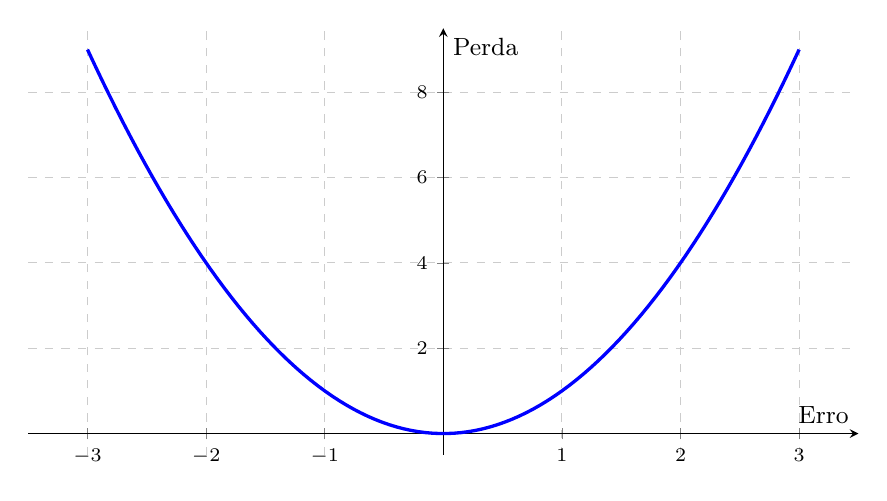
\begin{tikzpicture}
            \begin{axis}[
                % Dimensões ajustadas para caber lado a lado
                width=\linewidth,  
                height=7cm,
                xlabel={Erro},
                ylabel={Perda},
                axis lines=middle,
                grid=major,
                grid style={dashed, gray!40},
                xmin=-3.5, xmax=3.5,
                ymin=-0.5, ymax=9.5,
                legend pos=north west,
                title style={font=\bfseries\small},
                label style={font=\small},
                tick label style={font=\scriptsize}
            ]
                % Gráfico da função x^2
                \addplot[
                    domain=-3:3, 
                    samples=100, 
                    color=blue, 
                    very thick
                ] {x^2};

            \end{axis}
        \end{tikzpicture}
        \caption{Representação gráfica em duas dimensões da função criada.} % Legenda da subfigura
        \label{fig:mse-2d}
    \end{subfigure}
    \hfill % Adiciona espaço horizontal flexível entre as subfiguras
    % --- SUBFIGURA (b): NOVO GRÁFICO 3D ---
    \begin{subfigure}[b]{0.48\textwidth}
        \centering
        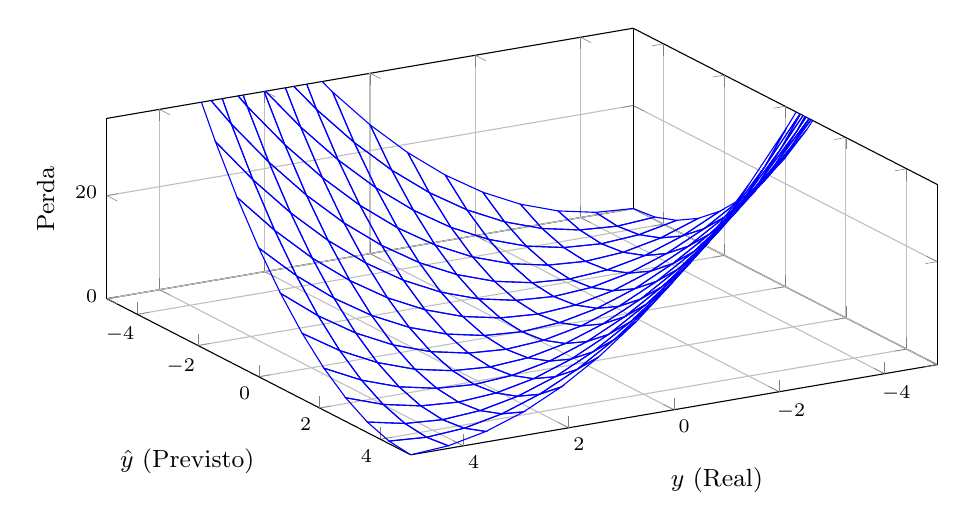
\begin{tikzpicture}
            \begin{axis}[
                % Dimensões consistentes com o gráfico (a)
                width=\linewidth,
                height=7cm,
                xlabel={$y$ (Real)},
                ylabel={$\hat{y}$ (Previsto)},
                zlabel={Perda},
                grid=major,
                view={150}{45}, % Ângulo de visão (azimute, elevação)
                zmin=0, zmax=35, % Ajuste o zmax conforme o domínio
                title style={font=\bfseries\small},
                label style={font=\small},
                tick label style={font=\scriptsize}
            ]
                % Gráfico da superfície (y - y_hat)^2, que é (x - y)^2 no pgfplots
                \addplot3[
                    mesh,           % Tipo de gráfico: superfície
                    color=blue,
                    shader=interp,  % Suaviza as cores
                    domain=-5:5,    % Domínio de x (y_real)
                    domain y=-5:5,  % Domínio de y (y_previsto)
                    samples=15      % Resolução da malha
                ] { (x - y)^2 }; % A função de perda MSE
            \end{axis}
        \end{tikzpicture}
        \caption{Representação gráfica em três dimensões da superfície criada.} % Legenda da subfigura
        \label{fig:mse-3d}
    \end{subfigure}

    % --- Legenda e Fonte da Figura Principal ---
    \caption{Visualizações da função de perda erro quadrático médio (\textit{MSE}) em duas e em três dimensões.}
    \label{fig:mse} % Rótulo principal da figura
    \fonte{O autor (2025).}
\end{figure}

\medskip
\begin{center}
 * * *
\end{center}
\medskip

\textbf{Características do Erro Quadrático Médio}
\vspace{1em}

Tendo os gráficos do erro quadrático médio além de sua equação, cabe agora discutir algumas das principais característica dessa função de perda.

\begin{itemize}
    \item \textbf{Não-negatividade:} Como é visto nos gráficos da Figura \ref{fig:mse}, o \textit{MSE} é uma função que retorna apenas valores positivos, isso se dá devido a diferença das entradas estar sendo calculada e logo em seguida elavada ao quadrado, impendido que valores negativos ocorram na saída;
    \item \textbf{Sensibilidade para \textit{outliers}:} Como \textcite{LossesArticle} discutem, a função erro quadrático médio possui a tendência de punir em maior força os erros que são originarios de uma distância muito grande. Isso acontece por conta do jeito que é calculada essa função, lembre que ela calcula a distância entre os pontos e depois eleva ela ao quadrado, se essa distância for muito grande, o erro será maior ainda. Como consequência, se existe um conjunto grande de pontos que ficam fora da regressão, os \textit{outliers}, a função de perda irá constamente retornar valores altos. Isso pode atrapalhar o aprendizado, porque será mais difícil otimizar o modelo, mas também pode ser uma vantagem em cenários em que os erros devem ser fortemente penalizados;
    \item \textbf{Convexa (nas predições):} Voltando para a Figura \ref{fig:mse} é possível notar que o \textit{MSE} é uma função convexa, o seu gráfico tem a típica forma de um funíl, apresentando um único ponto de mínimo global, isso ajuda na otimização dessa função caso se esteja usando um otimizador baseado no gradiente descendente. Contudo, \textcite{LossesArticle} destacam que em redes neurais profundas essa função pode se tornar não-convexa, devido as transformações não-lineares que são feitas ao construir o modelo;
    \item \textbf{Baixa intepretabilidade:} Note que a função \textit{MSE} eleva o erro ao quadrado, de forma que ao mostrar a perda não é visto diretamente a distância entre os pontos reais e os pontos preditos pelo modelo. Isso um gera um gargalo pois não é possível de forma instânea saber exatamente quão bem ou mal o modelo está performando. Funções como a \textit{MAE}, em que o erro é calculado como o módulo da distância entre os dois pontos são mais diretas em mostrar a performance do modelo;
    \item \textbf{Continuidade:} Ainda nos gráficos da Figura \ref{fig:mse} é possível notar que o \textit{MSE} é uma função contínua em todo o seu domínimo, isso é uma vantagem muito boa, pois indica que é possível derivar essa função sem encontrar grandes problemas.
\end{itemize}

\medskip
\begin{center}
 * * *
\end{center}
\medskip

Além disso, cabe também destacar a derivada da função \textit{MSE}, a qual está presente na Equação \ref{eq:mse-derivada}. A derivada de uma função de perda é de extrema utilizada para uma rede neural, pois é a partir dela que é calculado o primeiro vetor gradiente, e passa a ser retropropagado por toda a rede no sentido inverso, indo primeiro das últimas camadas para as camadas de entrada.

\begin{equacaodestaque}{Derivada Parcial do Erro Quadrático Médio (\textit{MSE}) em Relação a $\hat{y}_j$}
    \frac{\partial \Loss_{\text{MSE}}}{\partial \hat{y}_j} = \frac{2}{N}(\hat{y}_j - y_j)
    \label{eq:mse-derivada}
\end{equacaodestaque}

Note que diferente das funções de ativação em que era calculada a sua derivada ordinária, aqui é calculado as derivadas parciais das funções de perda para cada um dos seus componentes, a saída do modelo $\hat{y}_j$ e a saída esperada $y_j$. Com base nessas duas derivadas, é possível construir o vetor gradiente, como mostrado na Equação \ref{eq:vetor-gradiente-mse} \footnote{Perceba então que para ter o vetor gradiente completo, deve-se calcular a derivada parcial do \textit{MSE} também em relação os valor real do rótulo ($y_j$). Neste livro será dado um foco maior em apresentar apenas uma das derivas, pois elas muitas vezes apresentarão grandes semelhanças.}.

\begin{equation}
    \nabla (y_j, \hat{y}_j) = \left( \frac{\partial \Loss_{\text{MSE}}}{\partial y_j}, \frac{\partial \Loss_{\text{MSE}}}{\partial \hat{y}_j} \right)
    \label{eq:vetor-gradiente-mse}
\end{equation}

Considerando a derivada parcial da Equação \ref{mse-derivada}, é possível contruir gráficos como os da Figura \ref{eq:mse-derivada} para a derivada parcial do \textit{MSE} em relação a $(\hat{y}_j)$. Note também que semelhante as representações do erro quadrático médio, a sua derivada também é apresentada em vistas em duas e três dimensões, isso será algo recorrente nas representações das funções desse capítulo.

\begin{figure}[h!]
    \centering % Centraliza a figura na página

    % --- SUBFIGURA (a): Gráfico 2D da Derivada do MSE ---
    \begin{subfigure}[b]{0.48\textwidth}
        \centering
        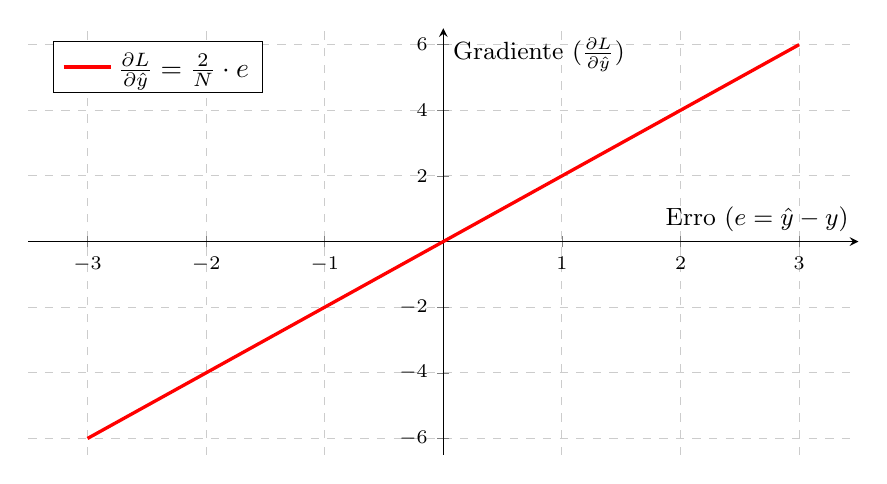
\begin{tikzpicture}
            \begin{axis}[
                % Dimensões ajustadas para caber lado a lado
                width=\linewidth,  
                height=7cm,
                xlabel={Erro ($e = \hat{y} - y$)},
                ylabel={Gradiente ($\frac{\partial L}{\partial \hat{y}}$)},
                axis lines=middle,
                grid=major,
                grid style={dashed, gray!40},
                xmin=-3.5, xmax=3.5,        % Limites do seu gráfico
                ymin=-6.5, ymax=6.5,         % Limites do seu gráfico
                legend pos=north west,
                title style={font=\bfseries\small},
                label style={font=\small},
                tick label style={font=\scriptsize}
            ]
                % Gráfico da função 2*x
                \addplot[
                    domain=-3:3, 
                    samples=100, 
                    color=red, 
                    very thick
                ] {2*x};
                
                % Mantendo sua legenda (com o fator 1/N)
                \addlegendentry{$\frac{\partial L}{\partial \hat{y}} = \frac{2}{N} \cdot e$}
            \end{axis}
        \end{tikzpicture}
        \caption{Visão 2D (Gradiente vs. Erro).} % Legenda da subfigura
        \label{fig:mse-derivada-2d}
    \end{subfigure}
    \hfill % Adiciona espaço horizontal flexível entre as subfiguras
    % --- SUBFIGURA (b): Gráfico 3D da Derivada do MSE ---
    \begin{subfigure}[b]{0.48\textwidth}
        \centering
        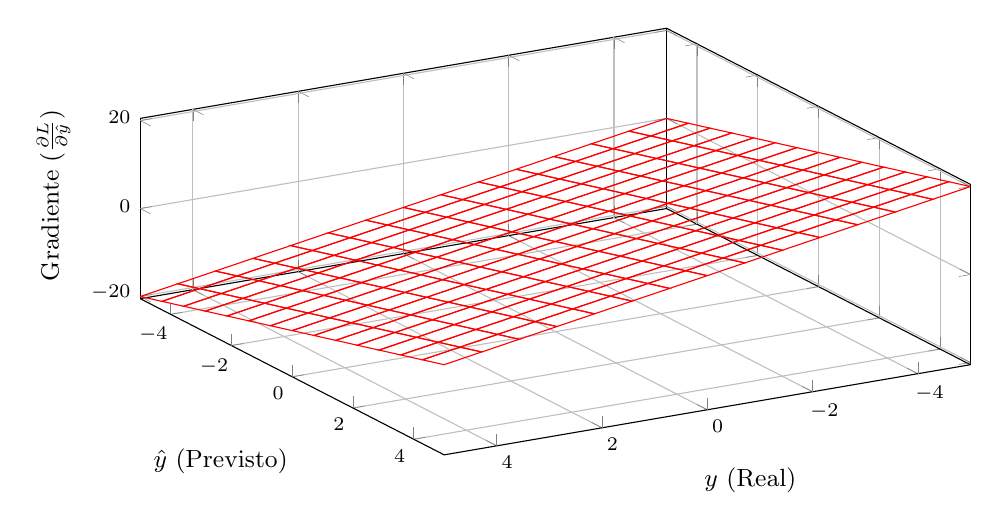
\begin{tikzpicture}
            \begin{axis}[
                % Dimensões consistentes com o gráfico (a)
                width=\linewidth,
                height=7cm,
                xlabel={$y$ (Real)},
                ylabel={$\hat{y}$ (Previsto)},
                zlabel={Gradiente ($\frac{\partial L}{\partial \hat{y}}$)},
                grid=major,
                view={150}{45}, % Mesmo ângulo de visão do seu template
                zmin=-20.5, zmax=20.5, % Ajustado para 2 * (erro máx 10)
                title style={font=\bfseries\small},
                label style={font=\small},
                tick label style={font=\scriptsize}
            ]
                % Gráfico da superfície do gradiente: 2 * (y_hat - y)
                \addplot3[
                    mesh,           
                    color=red,      % Cor consistente com o gráfico 2D
                    shader=interp,  
                    domain=-5:5,    % Mesmo domínio do seu template
                    domain y=-5:5,  % Mesmo domínio do seu template
                    samples=15      % Mesma resolução da malha
                ] { 2 * (y - x) }; % A função da derivada: 2 * (y_previsto - y_real)
            \end{axis}
        \end{tikzpicture}
        \caption{Superfície 3D completa.} % Legenda da subfigura
        \label{fig:mse-derivada-3d}
    \end{subfigure}

    % --- Legenda e Fonte da Figura Principal ---
    \caption{Visualizações da derivada (gradiente) da função de perda MSE.}
    \label{fig:mse-derivada} % Rótulo principal do seu gráfico
    \fonte{O autor (2025).}
\end{figure}

É possível perceber pelo gráfico da derivada da função de perda erro quadrático médio que o gradiente da perda é proporcional ao erro. Seguindo essa lógica, se o erro está alto, o gradiente também estará alto, como consequência as atualizações de pesos e vieses, as quais seguem o método do gradiente (visto nas Equações \ref{eq:gradiente-do-erro-em-relacao-a-um-peso-de-um-neuronio-regressao}) serão mais bruscas, dando maiores saltos no gráfico da função de perda. Enquanto em situações que o erro está pequeno em magnitudade, o gradiente também será pequeno e o modelo fará pequenas atualizações nos seus parâmetros, garantindo um ajuste fino.

\begin{equation}
    \frac{\partial E}{\partial w_{ji}} = \frac{\partial E}{\partial x_j} \cdot y_i \quad \text{ou} \quad \frac{\partial E}{\partial w_{ji}} = \frac{\partial E}{\partial y_j} \cdot \sigma'(x_j) \cdot y_i
    \label{eq:gradiente-do-erro-em-relacao-a-um-peso-de-um-neuronio-perda-regressao}
\end{equation}

\medskip
\begin{center}
 * * *
\end{center}
\medskip

\textbf{Algumas Aplicações do Erro Quadrático Médio em Problemas de Regressão}
\vspace{1em}

Além de estar presente nas deduções do algoritmo da retropropagação como uma função de perda, o erro quadrático médio acaba sendo uma função bem versátil para ser aplicada em problemas de regressão. Não somente isso, mas seu uso não se restringe a somente uma função de perda que será utilizada como "mapa" para a otimização do modelo, o \textit{MSE} também é uma ótima métrica para avaliar o desempenho de um modelo de regressão. E junto do \textit{MSE} está o \textit{RMSE}, cujo o cálculo é dado pela raíz quadrada do erro quadrático médio. Juntas, essas duas funções se tornam ótimas escolhas para medir como um modelo está performando.

Dito, isso, vale apenas destacar alguns desses cenários em que o erro quadrático médio é utilizado tanto como função de perda, quanto como métrica avaliativa. Além disso, é possível notar que muitas vezes ele irá aparecer indiretamente em formato de raíz do erro quadrático médio.

Assim, algumas aplicações do \textit{MSE} são:

\begin{itemize}
    \item \textbf{Estimação de custos médicos (Saúde):} Em \textit{Medical Costs Estimation Using Linear Regression Method}, \textcite{MedicalCostsEstimationUsingLR} utilizam técnicas de regressão linear como a regressão linear múltipla para fazer previsões de custos médicos. Para avaliar os modelos de regressão criados, os autores fazem uso do erro quadrático médio mas também aplicam outras métricas, como o erro absoluto médio (tópico principal da Seção xx), e também a métrica $R^2$ \parencite{MedicalCostsEstimationUsingLR};
    \item \textbf{Estimação de Preços de Imóveis (Mercado Imobiliário):} No artigo \textit{An Optimal House Price Prediction Algorithm: XGBoost}, \textcite{OptimalHousePricePrediction} aplicam diferentes modelos de regressão (como regressão linear, florestas aleatórias e XGBoost) com intuito de criar um modelo ideal para a prever valores de casas. Com esses diferentes modelos criados, os autores precisaram de diversas métricas para encontrar o modelo ideal, para isso, uma das técnicas foi o uso do \textit{MSE}, além disso, eles utilizam também o \textit{RMSE}, que é dado pelo cálculo da raíz quadrada do próprio erro quadrático médio \parencite{OptimalHousePricePrediction};
    \item \textbf{Previsão da Produção Agrícola (Agronomia):} No trabalho \textit{Coupling Machine Learning and Crop Modeling Improves Crop Yield Prediction in the US Corn Belt}, \textcite{CouplingMachineLearningAndCropModeling} estavam estudando formas de combinar técnicas com modelamento de culturas para prever a produção das plantações na regiaão do cinturação do milho nos Estados Unidos. No artigo, os pesquisadores não utilizam diretamente o \textit{MSE}, ao invés disso, utilizam a raíz do erro quadrático médio como uma das diferentes métricas para avaliação dos modelos de previsão desenvolvidos ao longo do projeto \parencite{CouplingMachineLearningAndCropModeling};
    \item \textbf{Previsão de Demanda de Energia (Gestão Energética):} Já no texto \textit{Optimizing Federated Learning for Scalable Power-demand Forecasting in Microgrids} ocorre uma situação diferente ao aplicar o erro quadrático médio, \textcite{OptimizingFL} fazem uma adptação nessa função transformando-a no \textit{Exponentially Weighted Mean Squared Error} (\textit{EW-RSM}). Essa adptação é justificada pelos autores como uma forma de enfatizar a acurácia em previsões de longo prazo atribuindo pesos exponencialmente crescentes aos erros em etapas de tempo posteriores \parencite{OptimizingFL}.
\end{itemize}

\medskip
\begin{center}
 * * *
\end{center}
\medskip

Conhecendo a função de perda \textit{MSE}, é possível agora discutir uma outra abordagem para resolver problemas de regressão. Para isso, a próxima seção busca apresentar o erro absoluto médio, que é uma alternativa para o erro quadrático médio que tem como principal diferença o jeito que lida com \textit{outliers}.

\subsection{Erro Absoluto Médio (MAE)}

O erro absoluto médio, também chamado de perda L1, é uma função que tem o mesmo propósito do erro quadrático médio, ser utilizada para tarefas de regressão. Neste caso o \textit{MAE} não possui uma origem definida que como o \textit{MSE}, esse conceito de minimizar a diferença de um resultado pelo seu valor real já havia sendo utilizado a bastante tempo. Contudo, trabalhos como \textit{Greedy function approximation: A gradient boosting machine} de \textcite{GreedyFunctionApproximation} fazem uso do erro absoluto médio para resolver problemas de aprendizado de máquina. No texto, o autor desenvolve um algoritmo de \textit{boosting} específico para o \textit{MAE}, neste caso, essa função é apresentada com outro nome, \textit{Least-Absolute-Deviation} (\textit{LAD}), sendo responsável por dar nome ao algoritmo criado, o \texttt{LAD\_TreeBoost} \parencite{GreedyFunctionApproximation}. Neste caso, \textcite{GreedyFunctionApproximation} explica que esse algoritmo faz uso de uma árvore de regressão com a perda, de forma que para prever a pseudo-resposta que é o sinal dos resíduos atuais é utilizado o método dos mínimos quadrados. Assim, o modelo é atualizado adicionando em cada nó terminal da nova árvore criada a mediana dos resíduos daquela região específica.

Um trabalho mais recente que explora o uso dessa função é o \textit{Image-to-Image Translation with Conditional Adversarial Networks} \parencite{ImageToImage}. Nele, \textcite{ImageToImage} argumentam que preferiram trabalhar com a função de perda \textit{L1 distance} (um dos diferentes nomes utilizados para se referir ao \textit{MAE}) devido a essa função gerar imagens menos borradas. É possível ver essa comparação nas imagens da Figura \ref{fig:comparativo-perdas-image-to-image}. Perceba que a perda que apresenta os resultados mais consistentes com a realidade é justamente a \textit{L1 + cGAN}, a qual possuí o \textit{MAE} em sua composição.

\begin{figure}[h]
    \centering
    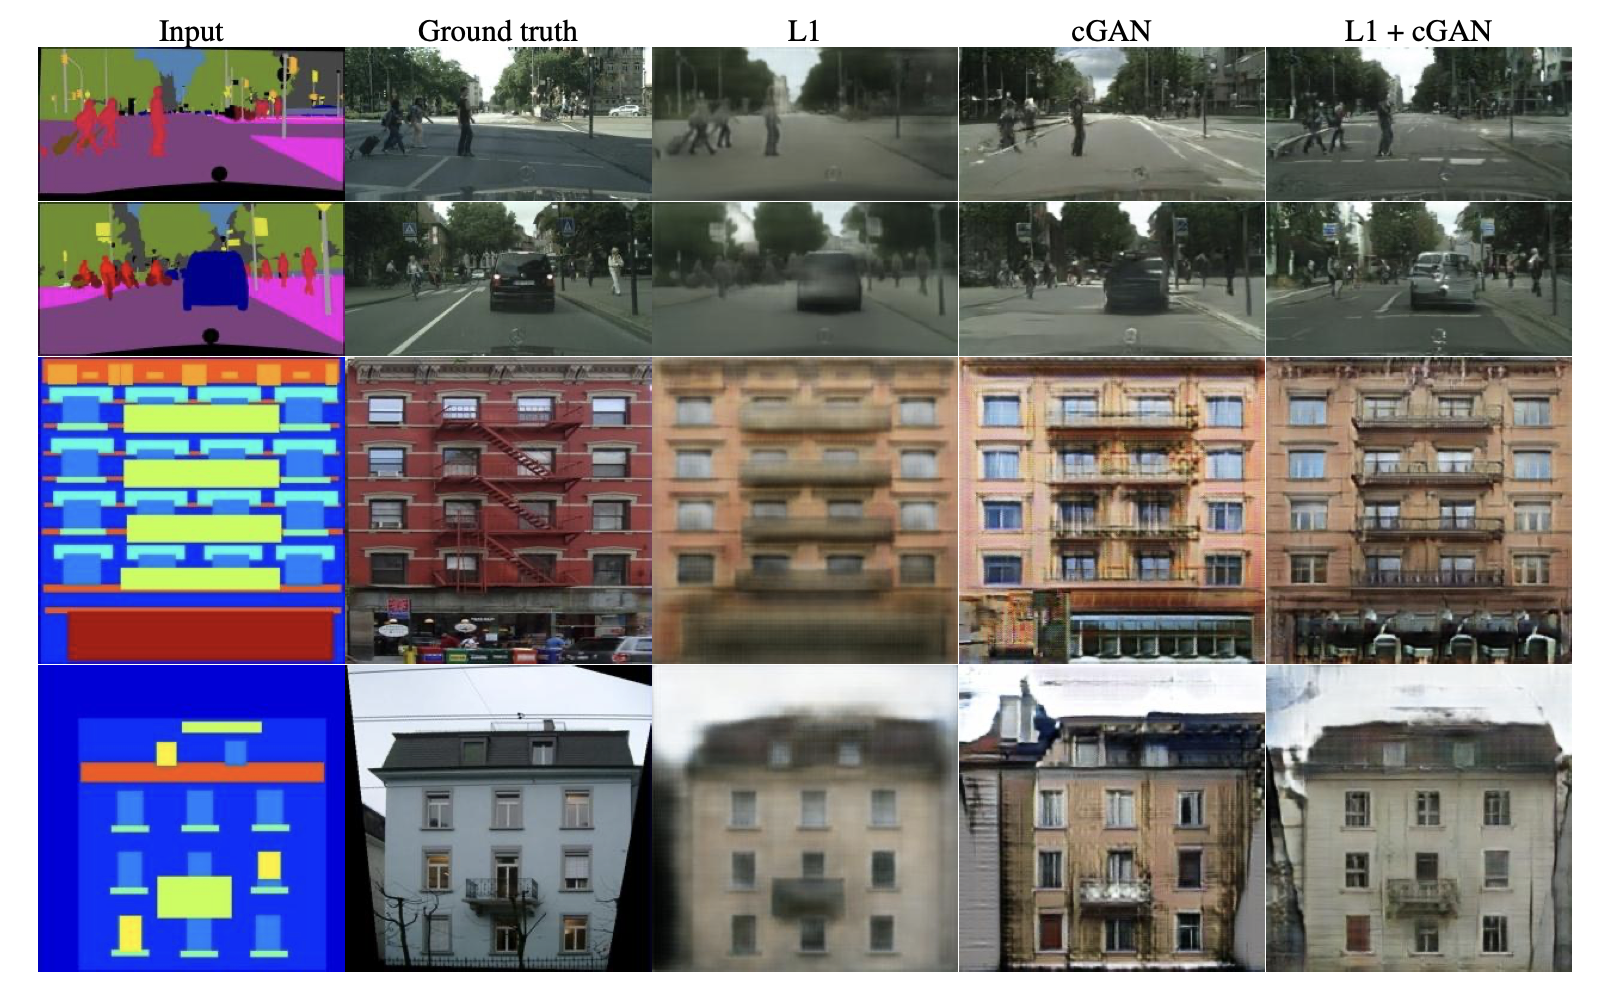
\includegraphics[width=0.65\linewidth]{../imagens/perda-regressao/image-to-image-perdas-comparativo.png}
    
    \caption[Perdas diferentes induzem qualidades de resultados diferentes. Cada coluna mostra resultados treinados sob uma perda diferenteas de aprendizado no dataset MNIST]{%
        \newline
        \small Fonte: \parencite{ImageToImage}.
    }
    \label{fig:comparativo-perdas-image-to-image}
\end{figure}

Além disso, vale a pena destacar como o erro absoluto médio se enquadra no exemplo ilustrativo do jogo dos dardos. Para isso, diferente do erro quatrático médio, em que quanto mais longe do centro, o número de pontos perdidos aumentava de forma quadrática, no \textit{MAE} a penalização com relação aos jogadores ruins é mais suave, sendo dada de forma linear. 

Além disso, é interessante fazer uma outra analogia considerando o cenário em que o \textit{MAE} se encontra. Para isso, é preciso considerar que será feito um novo jogo de dardos com dez participantes, em que cada um tem direito de jogar apenas um dardo, e que no final os dez dardos serão somados e com base neles será dado o resultado da equipe. Se tivéssemos uma equipe muito ruim utilizando como métrica o \textit{MSE} para avaliar os pontos, o resultado seria péssimo, porque esses dardos estariam muito longes do centro, e como o erro é elevado ao quadrado, isso geraria uma pontuação muito baixa. 

Contudo, se a métrica escolhida para avaliar o jogo fosse o \textit{MAE} o resultado seria bem melhor, visto que o erro cresce de forma linear. Saindo da alogia e voltando para o cenário de aprendizado de máquina, é possível associar os jogadores ruins com os \textit{outliers}, eles estão presentes nos dados e vão atrapalhar o aprendizado do seu modelo. Contudo, escolher uma função que não seja tão agressiva na medição desses \textit{outliers} pode ser uma excelente alternativa para trabalhar em cenários em que essa configuração será muito comum.

Visto esses diferentes cenários em que o erro absoluto médio foi utilizado para resolver problemas de regressão, além de como ele pode ser associado com o jogo dos dardos, é possível ver agora a sua definição matemática. Para isso, o \textit{MAE} está definido na Equação \ref{eq:mae}. Perceba que ele é responsável por calcular a diferença entre os dois pontos, o valor real $\hat{y}_j$ e o valor predito $y_j$, para todos os $N$ casos analisados e a partir disso calcular a média dos resultados.

\begin{equacaodestaque}{Erro Absoluto Médio (\textit{MAE})}
    \Loss_{\text{MAE}} = \frac{1}{N} \sum_{j=1}^{N} |y_j - \hat{y}_j|
    \label{eq:mae}
\end{equacaodestaque}


Também vale a pena analisar o erro absoluto médio de forma gráfica. Para isso, suas representações em duas e três dimensões estão presentes na Figura \ref{fig:mae} de forma semelhante ao que foi feito ao apresentar o \textit{MSE}.

\begin{figure}[h!]
    \centering % Centraliza a figura na página

    % --- SUBFIGURA (a): Gráfico 2D do MAE ---
    \begin{subfigure}[b]{0.48\textwidth}
        \centering
        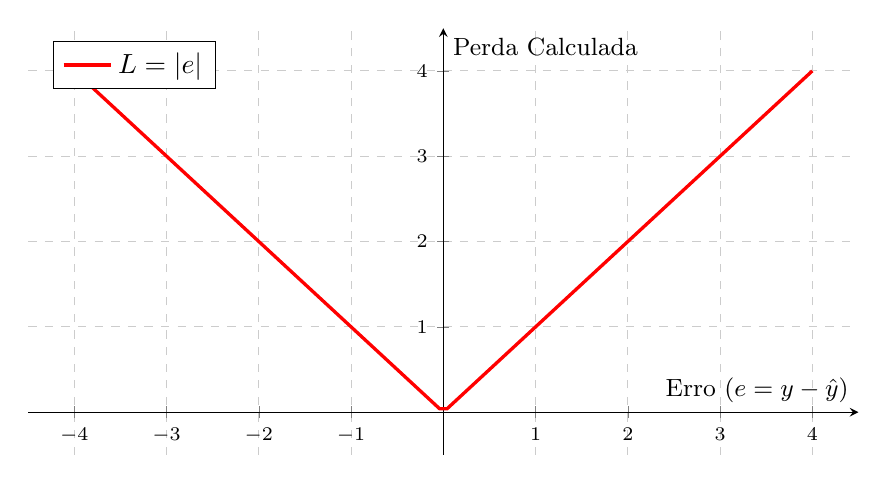
\begin{tikzpicture}
            \begin{axis}[
                % Dimensões ajustadas para caber lado a lado
                width=\linewidth,  
                height=7cm,
                xlabel={Erro ($e = y - \hat{y}$)},
                ylabel={Perda Calculada},
                axis lines=middle,
                grid=major,
                grid style={dashed, gray!40},
                xmin=-4.5, xmax=4.5,        % Limites do seu gráfico MAE
                ymin=-0.5, ymax=4.5,         % Limites do seu gráfico MAE
                legend pos=north west,
                title style={font=\bfseries\small},
                label style={font=\small},
                tick label style={font=\scriptsize}
            ]
                % Gráfico da função abs(x)
                \addplot[
                    domain=-4:4, 
                    samples=100, 
                    color=red, 
                    very thick
                ] {abs(x)};
                
                \addlegendentry{$L = |e|$}
            \end{axis}
        \end{tikzpicture}
        \caption{Representação gráfica em duas dimensões.} % Legenda da subfigura
        \label{fig:mae-2d}
    \end{subfigure}
    \hfill % Adiciona espaço horizontal flexível entre as subfiguras
    % --- SUBFIGURA (b): Gráfico 3D do MAE ---
    \begin{subfigure}[b]{0.48\textwidth}
        \centering
        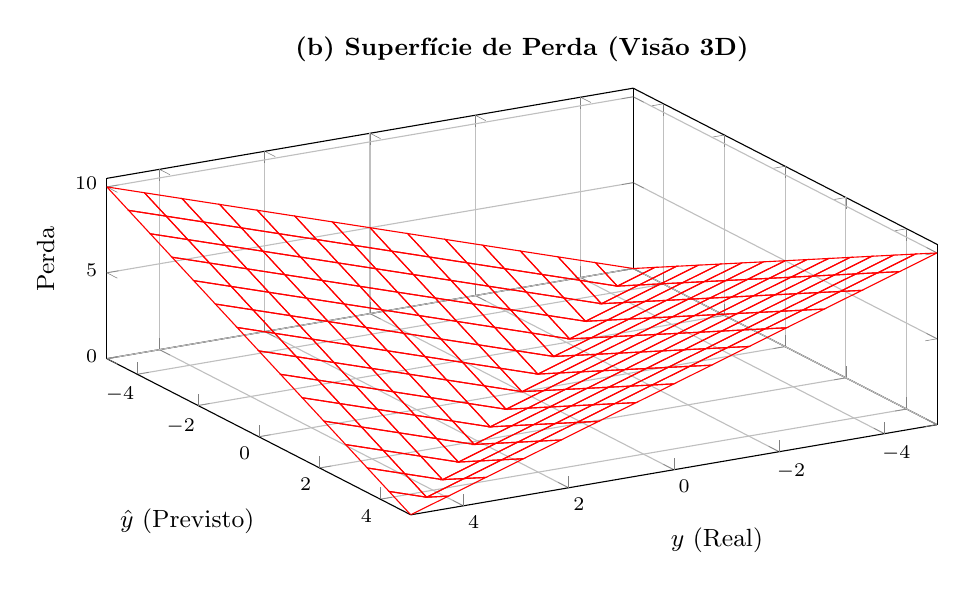
\begin{tikzpicture}
            \begin{axis}[
                % Dimensões consistentes com o gráfico (a)
                width=\linewidth,
                height=7cm,
                title={(b) Superfície de Perda (Visão 3D)},
                xlabel={$y$ (Real)},
                ylabel={$\hat{y}$ (Previsto)},
                zlabel={Perda},
                grid=major,
                view={150}{45}, % Mesmo ângulo de visão do seu template
                zmin=0, zmax=10.5, % Limite Z ajustado para o MAE (abs(-5 - 5) = 10)
                title style={font=\bfseries\small},
                label style={font=\small},
                tick label style={font=\scriptsize}
            ]
                % Gráfico da superfície abs(y - y_hat)
                \addplot3[
                    mesh,           
                    color=red,      % Cor consistente com o gráfico 2D
                    shader=interp,  
                    domain=-5:5,    % Mesmo domínio do seu template
                    domain y=-5:5,  % Mesmo domínio do seu template
                    samples=15      % Mesma resolução da malha
                ] { abs(x - y) }; % A função de perda MAE
            \end{axis}
        \end{tikzpicture}
        \caption{Representação gráfica em três dimensões.} % Legenda da subfigura
        \label{fig:mae-3d}
    \end{subfigure}

    % --- Legenda e Fonte da Figura Principal ---
    \caption{Visualizações da função de perda erro absoluto médio (\textit{MAE}) em duas e em três dimensões.}
    \label{fig:mae} % Rótulo principal do seu gráfico MAE
    \fonte{O autor (2025).}
\end{figure}

\medskip
\begin{center}
 * * *
\end{center}
\medskip

\textbf{Características do Erro Absoluto Médio}
\vspace{1em}

A partir do seu gráfico e de sua equação é possível retirar diferentes informações dessa função de perda, as quais estão discutidas a seguir:

\begin{itemize}
    \item \textbf{Não-negatividade:} Como é possível ver em seu gráfico da Figura \ref{fig:mae}, o erro absoluto médio compartilha dessa mesma propriedade com o \textit{MSE}, isso significa que sua saída será sempre positiva ou zero, independente do valor de entrada. Isso se dá, devido a propriedade do módulo, que não admite números negativos para sua saída;
    \item \textbf{Robustez para \textit{outliers}}: Como \textcite{LossesArticle} explicam, o \textit{MAE} não penaliza os \textit{outliers} de forma tão severa como o erro quadrático médio. Isso acontece pois diferente do \textit{MSE}, em que o erro cresce de forma quadrática, no \textit{MAE}, ele cresce de forma linear, significando que diferente do \textit{MSE} que era sensível aos \textit{outliers}, o \textit{MAE} também reage à eles, mas de forma menos severa;
    \item \textbf{Convexa (nas predições):} Voltando para o seu gráfico, é possível ver que o erro absoluto médio segue a mesma forma de funíl do erro quadrático médio, podendo ser considerado uma função convexa e com um só ponto de mínimo global. Contudo, assim como no \textit{MSE}, \textcite{LossesArticle} advertem que para modelos de apredenziado profundo, o \textit{MAE} pode deixar de ser uma função convexa devido às muitas camadas e funções não-lineares;
    \item \textbf{Não-derivável em zero:} Esse ponto acontece justamente devido a forma que a função apresenta, ela faz uma especíe de "bico" em zero, além disso, ao calcular os seus limites laterais para verificar a continuidade da função é possível notar que eles apresentam valores diferentes;
    \item \textbf{Boa intepretabilidade:} Diferente do erro quadrático médio em que o erro total é elevado ao quadrado, no \textit{MAE} isso não ocorre, o erro é simplemente a média das diferenças dos pontos. Isso significa que é mais fácil interpretar os resultados que essa função de perda retorna, pois não é preciso fazer nenhum cálculo adicional para ter uma ideia precisa se as previsões feitas pelo modelo estão longe ou não dos valores reais;
\end{itemize}

\medskip
\begin{center}
 * * *
\end{center}
\medskip

Como foi destacado anteriormente, o \textit{MAE} não é derivável em zero. Inicialmente pode ter-se a ideia de que devido a isso, essa não seja uma função boa para ser utilizada em conjunto com otimizadores baseados em gradiente, porque pontos de descontinuidade como este podem acabar atrapalhando a forma como o molode é otimizado. Contudo, \textcite{LossesArticle} argumentam, é possível resolver esse problema utilizado técnicas de subgradiente, sendo possível então escrever a derivada do \textit{MAE} com a Equação \ref{eq:mae-derivada}.

\begin{equacaodestaque}{Derivada Parcial do Erro Absoluto Médio (\textit{MAE}) em Relação a $\hat{y}_j$}
    \frac{\partial \Loss_{\text{MAE}}}{\partial \hat{y}_j} = 
    \begin{cases} 
      -1 & \text{se } \hat{y}_j > y_j \\
      +1 & \text{se } \hat{y}_j < y_j \\
      [-1, +1] & \text{se } \hat{y}_j = y_j
    \end{cases}
    \label{eq:mae-derivada}
\end{equacaodestaque}

Contudo, mesmo possuindo esse detalhe de descontinuidade em zero, isso não atrapalha a plotagem do gráfico do \textit{MAE}, o qual está representado na Figura \ref{fig:mae-derivada}. De forma semelhante ao que foi feito até agora, na figura da esquerda, a Figura \ref{fig:mae-derivada-2d}, está a representação em duas dimensões dessa função, enquanto na figura da direta, a Figura \ref{fig:mae-derivada-3d}.

\begin{figure}[h!]
    \centering % Centraliza a figura na página

    % --- SUBFIGURA (a): Gráfico 2D da Derivada do MAE ---
    \begin{subfigure}[b]{0.48\textwidth}
        \centering
        \begin{tikzpicture}
            \begin{axis}[
                % Dimensões ajustadas para caber lado a lado
                width=\linewidth,  
                height=7cm,
                xlabel={Erro ($e = \hat{y} - y$)},
                ylabel={Gradiente ($\frac{\partial L}{\partial \hat{y}}$)},
                axis lines=middle,
                grid=major,
                grid style={dashed, gray!40},
                xmin=-3.5, xmax=3.5,        % Limites do seu gráfico
                ymin=-1.5, ymax=1.5,         % Limites do seu gráfico
                ytick={-1, 0, 1},           % Pontos no eixo y
                legend pos=north west,
                title style={font=\bfseries\small},
                label style={font=\small},
                tick label style={font=\scriptsize}
            ]
                % Parte negativa da derivada (-1)
                \addplot[
                    domain=-3:0, 
                    samples=100, 
                    color=red, 
                    very thick
                ] {-1};

                % Parte positiva da derivada (+1)
                \addplot[
                    domain=0:3, 
                    samples=100, 
                    color=red, 
                    very thick
                ] {1};
                
                % Círculos abertos para a descontinuidade em x=0
                \addplot[only marks, mark=o, color=red, mark size=2pt] coordinates {(0,-1) (0,1)};
            \end{axis}
        \end{tikzpicture}
        \caption{Visão 2D (Gradiente vs. Erro).} % Legenda da subfigura
        \label{fig:mae-derivada-2d}
    \end{subfigure}
    \hfill % Adiciona espaço horizontal flexível entre as subfiguras
    % --- SUBFIGURA (b): Gráfico 3D da Derivada do MAE ---
    \begin{subfigure}[b]{0.48\textwidth}
        \centering
        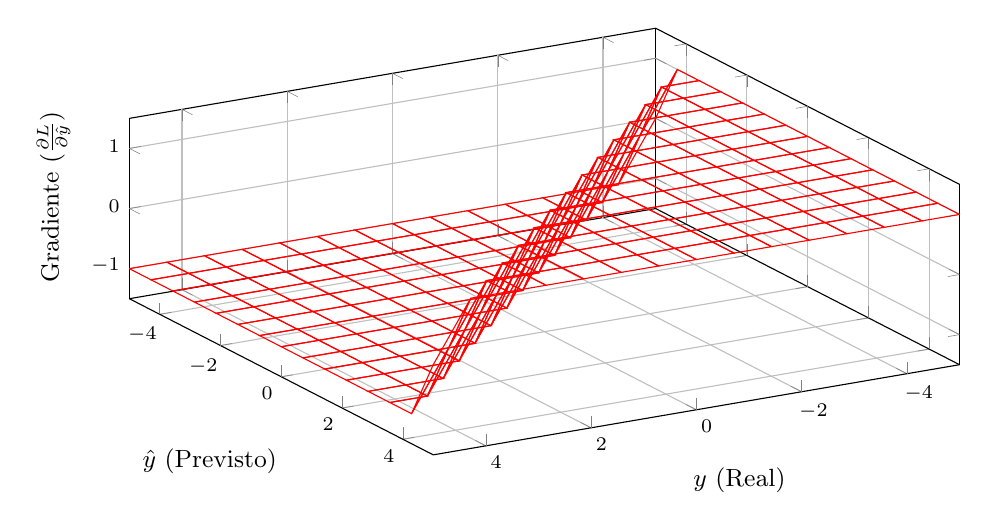
\begin{tikzpicture}
            \begin{axis}[
                % Dimensões consistentes com o gráfico (a)
                width=\linewidth,
                height=7cm,
                xlabel={$y$ (Real)},
                ylabel={$\hat{y}$ (Previsto)},
                zlabel={Gradiente ($\frac{\partial L}{\partial \hat{y}}$)},
                grid=major,
                view={150}{45}, % Mesmo ângulo de visão do seu template
                zmin=-1.5, zmax=1.5, % Espelha o eixo Y do gráfico 2D
                ztick={-1, 0, 1}, % Consistente com o 2D
                title style={font=\bfseries\small},
                label style={font=\small},
                tick label style={font=\scriptsize}
            ]
                % Gráfico da superfície do gradiente: sign(y_hat - y)
                \addplot3[
                    mesh,           
                    color=red,      % Cor consistente com o gráfico 2D
                    shader=interp,  
                    domain=-5:5,    % Mesmo domínio do seu template
                    domain y=-5:5,  % Mesmo domínio do seu template
                    samples=15      % Mesma resolução da malha
                ] { sign(y - x) }; % A função da derivada: sign(y_previsto - y_real)
            \end{axis}
        \end{tikzpicture}
        \caption{Superfície 3D completa.} % Legenda da subfigura
        \label{fig:mae-derivada-3d}
    \end{subfigure}

    % --- Legenda e Fonte da Figura Principal ---
    \caption{Visualizações da derivada (gradiente) da função de perda MAE.}
    \label{fig:mae-derivada} % Rótulo principal do seu gráfico
    \fonte{O autor (2025).}
\end{figure}

Perceba que a derivada do erro absoluto médio é representado em forma de uma função por partes, neste caso, ela é divida em duas diferentes retas, parecida com a função de ativação degrau unitário. Note também que existe um "bico" na união dessas duas retas, isso acontece devido a descontinuidade dessa função em zero, o que impede de ser derivada nesse ponto. Assim, a derivada do \textit{MAE} pode ser interpretada como a composição de duas retas constantes, a primeira constante em -1, e a segunda constante em 1.

\medskip
\begin{center}
 * * *
\end{center}
\medskip

\textbf{Algumas Aplicações do Erro Absoluto Médio em Problemas de Regressão}
\vspace{1em}

Além dos casos discutidos no início da seção: o \texttt{LAD\_TreeBoost} e o artigo \textit{Image-to-Image Translation with Conditional Adversarial Networks}, o \textit{MAE} também está presente em uma série de trabalhos, atuando tanto como função de perda, quanto servindo como uma métrica de avaliação, indicando se o modelo desenvolvido está performando bem ou não. Dito isso, essa seção busca explorar algumas dessas aplicações do erro absoluto médio, semelhante ao que foi feito ao analisar o erro quadrático médio. 

Dito isso, vale destacar os trabalhos:

\begin{itemize}
    \item \textbf{Avaliação de idade óssea e estimação do escore de cálcio na artéria coronária (Saúde):} Em \textit{Regression Metric Loss: Learning a Semantic Representation Space for Medical Images}, \textcite{chao2022regressionmetriclosslearning} desenvolvem algortimos de regressão para estimar escore de cálcio da artéria coronária e também um segundo algoritmo para avaliação da idade óssea. Além disso, os autores apresentam uma nova função de perda, a \textit{RM-Loss} que demonstra ser mais apta para resolver os problemas propostos de regressão \parencite{chao2022regressionmetriclosslearning}. Como forma de avaliar essa nova função criada e também as diferentes outras funções comparadas no artigo, \textcite{chao2022regressionmetriclosslearning} utilizam o erro absoluto médio como uma das métricas;
    \item \textbf{Restauração de imagens (Engenharia):} No artigo \textit{Noise2Noise: Learning Image Restoration without Clean Data}, \textcite{Noise2Noise} estavam estudando formas de restaurar imagens corrompidas sem a utilização de dados limpos. Em um dos experimentos os autores estavam buscando uma forma ideal de remover textos de imagens, de forma que a perda L1, por ser uma função de perda robusta, conseguiu atingir bons resultados nessa tarefa \parencite{Noise2Noise};
    \item \textbf{Previsão da produção de energia eólica (Setor energético):} Já em \textit{Minimum Open Data Subset for Wind Power Prediction}, \textcite{MinimumOpenDataSubsetForWindPowerPrediction} utilizam um modelo de florestas aleatórias com o objetivo de prever a produção de energia eólica. Para avaliar o modelo de regressão desenvolvido, os autores utilizam como métricas o \textit{MAE} além do \textit{RMSE}. Além disso, vale comentar que em testes realizados pelos pesquisadores foi possível criar um modelo com erro absoluto médio de 0,071, indicando um excelente resultado para para o algoritmo criado \parencite{MinimumOpenDataSubsetForWindPowerPrediction}.
    \item \textbf{Previsão de poluição do ar (Setor ambiental):} Por fim, vale a pena destacar o trabaho de \textcite{nedungadi2025aircastimprovingairpollution}, \textit{AirCast: Improving Air Pollution Forecasting Through Multi-Variable Data Alignment}, em que os autores buscam formas de melhorar a previsão da poluição do ar. Como forma de ajudar a resolver esse problema, os autores utilizam uma função inspirada pelo erro absoluto médio, o \textit{Frequency-weighted Mean Absolute Error} (\textit{fMAE}), que tem como principal vantagem lidar com variáveis que apresentam uma distribuição de cauda pesada, como as variáveis PM1, PM2.5 e PM10, que indicam a qualidade do ar \parencite{nedungadi2025aircastimprovingairpollution}.
\end{itemize}

\medskip
\begin{center}
 * * *
\end{center}
\medskip

Visto o erro quadrático médio, que penaliza fortamente ou \textit{outliers}, e o erro absoluto médio, que não penaliza de forma agressiva os \textit{outliers}, surge uma pergunta: Existe alguma forma de ter uma função que penalize os erros gravemente até um certo ponto e depois desse, ela não se preocupe tanto com os \textit{outliers}? Essa é a proposta da perda de Huber, a qual busca unir os principais benefícios dessas duas funções de regressão. Ela é o tópico principal da próxima seção.

\subsection{Perda de Huber}

A Huber \textit{Loss} recebe o seu nome devido ao seu criador, Peter J. Huber, que apresentou para a comunidade científica no trabalho \textit{Robust Estimation of a Location Parameter} \parencite{HuberLoss}. No artigo, \textcite{HuberLoss} define um estimador robusto $p$ que segue a Equação \ref{eq:huber-loss-do-huber}.

\begin{equation}
    p(t) = 
    \begin{cases}
        \frac{1}{2} t^2 \text{para} |t| < k \\
        k |t| - \frac{1}{2} k^2 para t \ge k
    \end{cases}
    \label{eq:huber-loss-do-huber}
\end{equation}

O que Huber estava querendo basicamente era uma função que se comportasse de forma quadrática para os casos em que $|t| < k$ e que se comportasse de forma linear para os casos em que $t \ge k$. Essa função criada pelo pesquisador é a função que está sendo estudada, a perda Huber, a qual pode ser representada, agora com notações voltadas para o cenário de aprendizado de máquina, com a Equação \ref{eq:huber-loss}.

\begin{equacaodestaque}{Huber Loss}
    \Loss_{\text{Huber}}(y, \hat{y}) = 
    \begin{cases} 
      \frac{1}{2}(y - \hat{y})^2 & \text{para } |y - \hat{y}| \le \delta \\
      \delta (|y - \hat{y}| - \frac{1}{2}\delta) & \text{caso contrário}
    \end{cases}
    \label{eq:huber-loss}
\end{equacaodestaque}

É possível também representar a perda Huber utilizando gráficos, para isso, ela pode ser vista na Figura \ref{fig:huber-loss}. Perceba que é como se ela fosse duas funções em uma, até um certo ponto do gráfico ela age parecido a uma função quadrática, contudo, após passar do limite de $\delta$ ela passa a ser uma função linear.

\begin{figure}[h!]
    \centering % Centraliza a figura na página

    % --- SUBFIGURA (a): Gráfico 2D da Huber Loss ---
    \begin{subfigure}[b]{0.48\textwidth}
        \centering
        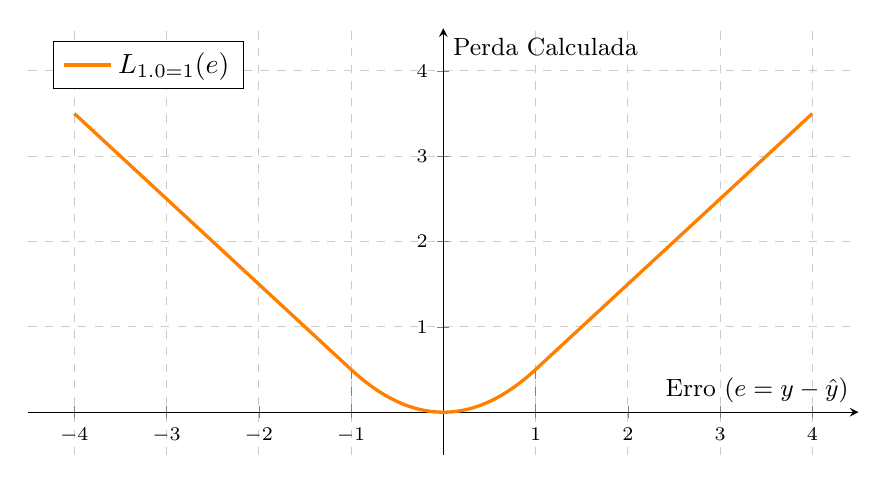
\begin{tikzpicture}
            % Define o valor de delta para este gráfico
            \def\delta{1.0} 
            
            \begin{axis}[
                % Dimensões ajustadas para caber lado a lado
                width=\linewidth,  
                height=7cm,
                xlabel={Erro ($e = y - \hat{y}$)},
                ylabel={Perda Calculada},
                axis lines=middle,
                grid=major,
                grid style={dashed, gray!40},
                xmin=-4.5, xmax=4.5,        % Limites do seu gráfico
                ymin=-0.5, ymax=4.5,         % Limites do seu gráfico
                legend pos=north west,
                title style={font=\bfseries\small},
                label style={font=\small},
                tick label style={font=\scriptsize}
            ]
                % Gráfico da função Huber Loss
                \addplot[
                    domain=-4:4, 
                    samples=201, 
                    color=orange, 
                    very thick
                ] { abs(x) <= \delta ? 0.5*x^2 : \delta*(abs(x) - 0.5*\delta) };
                
                \addlegendentry{$L_{\delta=1}(e)$}

                % Linhas de transição em delta
                \draw[dashed, gray] (axis cs:-\delta, 0) -- (axis cs:-\delta, {\delta*(\delta-0.5*\delta)});
                \draw[dashed, gray] (axis cs:\delta, 0) -- (axis cs:\delta, {\delta*(\delta-0.5*\delta)});
            \end{axis}
        \end{tikzpicture}
        \caption{Representação gráfica em duas dimensões.} % Legenda da subfigura
        \label{fig:huber-2d}
    \end{subfigure}
    \hfill % Adiciona espaço horizontal flexível entre as subfiguras
    % --- SUBFIGURA (b): Gráfico 3D da Huber Loss ---
    \begin{subfigure}[b]{0.48\textwidth}
        \centering
        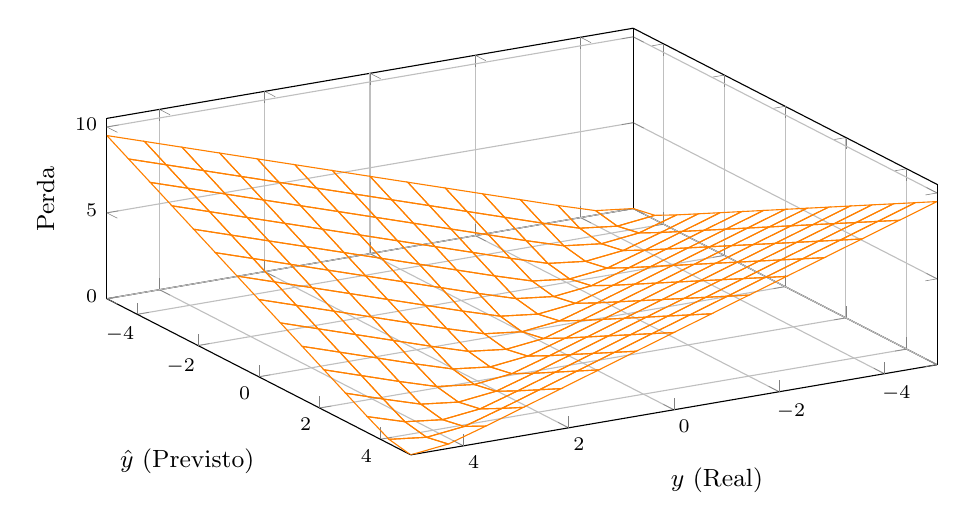
\begin{tikzpicture}
            % Define o valor de delta para este gráfico
            \def\delta{1.0}
            
            \begin{axis}[
                % Dimensões consistentes com o gráfico (a)
                width=\linewidth,
                height=7cm,
                xlabel={$y$ (Real)},
                ylabel={$\hat{y}$ (Previsto)},
                zlabel={Perda},
                grid=major,
                view={150}{45}, % Mesmo ângulo de visão do seu template
                zmin=0, zmax=10.5, % Limite Z ajustado para Huber com domínio -5:5
                title style={font=\bfseries\small},
                label style={font=\small},
                tick label style={font=\scriptsize}
            ]
                % Gráfico da superfície da Huber Loss
                \addplot3[
                    mesh,           
                    color=orange,   % Cor consistente com o gráfico 2D
                    shader=interp,  
                    domain=-5:5,    % Mesmo domínio do seu template
                    domain y=-5:5,  % Mesmo domínio do seu template
                    samples=15      % Mesma resolução da malha
                ] { abs(x-y) <= \delta ? 0.5*(x-y)^2 : \delta*(abs(x-y) - 0.5*\delta) }; % A função Huber 3D
            \end{axis}
        \end{tikzpicture}
        \caption{Representação gráfica em três dimensões.} % Legenda da subfigura
        \label{fig:huber-3d}
    \end{subfigure}

    % --- Legenda e Fonte da Figura Principal ---
    \caption{Visualizações da função de perda Huber (\textit{Huber Loss}, $\delta=1$) em duas e em três dimensões.}
    \label{fig:huber-loss} % Rótulo principal do seu gráfico
    \fonte{O autor (2025).}
\end{figure}

\medskip
\begin{center}
 * * *
\end{center}
\medskip

\textbf{Características da Perda de Huber}
\vspace{1em}

Conhecido o gráfico e sua equação, é possível agora discutir algumas das propriedades da perda huber, as quais são apresentadas a seguir:

\begin{itemize}
    \item \textbf{Robustez para \textit{outliers}:} Assim como o \textit{MAE}, a perda Huber não penaliza de forma quadrática os erros como comparado com o erro quadrático médio, dessa forma, os \textit{outliers} não conseguem afetar desticmaente o cálculo da perda dependendo do valor de $\delta$ escolhido \parencite{LossesArticle}.
    \item \textbf{Diferenciabilidade em $\delta$:} Um ponto a ser destacado ao se utilizar a perda Huber é que ela apresenta pontos de descontinuidade para o cenário em que $y - \hat{y} = \delta$, contudo a função é contínua em todo o resto, dessa forma, isso não a impede de ser utilizada em conjunto com otimizadores baseados em gradiente \parencite{LossesArticle}.
\end{itemize}

\medskip
\begin{center}
 * * *
\end{center}
\medskip

O gradiente da perda Huber deve ser calculado por partes, como explicam \textcite{LossesArticle}, para isso, é possível utilizar a Equação \ref{eq:huber-loss-derivada} como guia.

\begin{equacaodestaque}{Huber Loss Derivada}
    \frac{\partial \Loss_{\delta}}{\partial \hat{y}} = 
    \begin{cases} 
        \hat{y} - y & \text{se } | y - \hat{y} | \le \delta \\
        \delta \cdot \text{sgn}(\hat{y} - y) & \text{se } | y - \hat{y} | > \delta
    \end{cases}
    \label{eq:huber-loss-derivada}
\end{equacaodestaque}

Um ponto a ser destacado ao utilizar a Huber \textit{loss} é com relação a escolha de valores para o parâmetro $\delta$. Um valor muito pequeno para $\delta$ faz com que a função se comporte mais como o erro absoluto médio, é possível ver essa situação na Figura \ref{fig:huber-comparacoes-mae}, já ao escolher um valor muito grande para $\delta$ faz com que a perda Huber se assemelhe mais a função erro quadrático médio, essa sitação está na Figura \ref{fig:huber-comparacoes-mse}. \textcite{LossesArticle} explicam que a escolha de valores para $\delta$ pode ser feita de forma empírica, através de validação cruzada (\textit{cross-validation}). Assim, testes são recomendados a fim de escolher o melhor valor para $\delta$ no cenário em que está sendo trabalhado.

\begin{figure}[h!]
    \centering
    % Figura da Esquerda (Parecida com MAE)
    \begin{subfigure}[b]{0.48\textwidth}
        \centering
        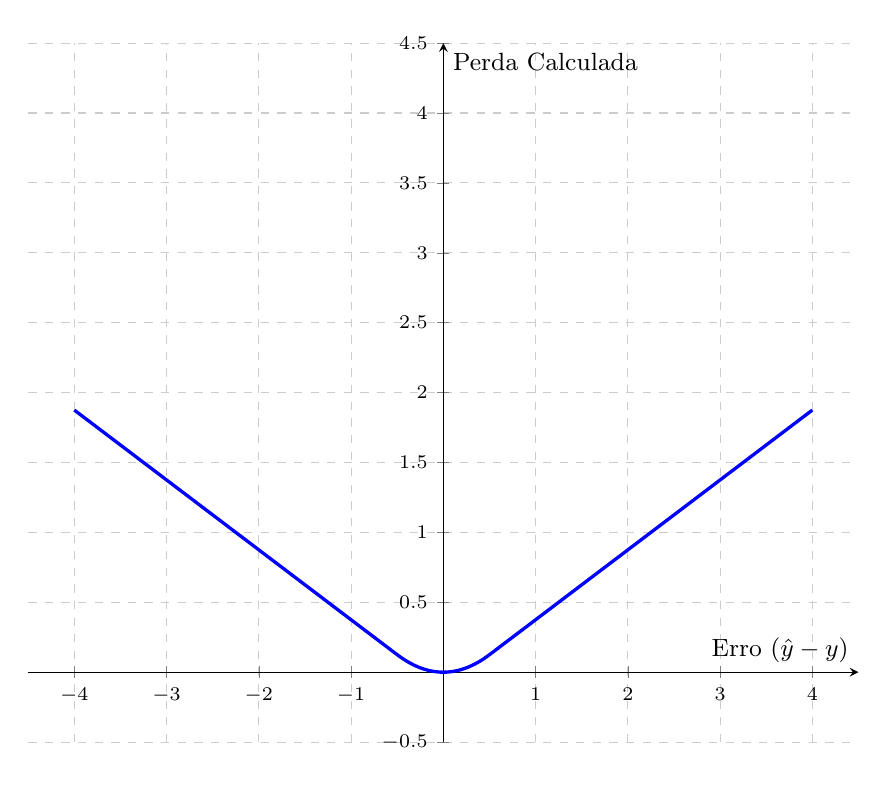
\begin{tikzpicture}
            \def\delta{0.5} % Delta pequeno
            \begin{axis}[
                xlabel={Erro ($\hat{y} - y$)},
                ylabel={Perda Calculada},
                axis lines=middle,
                grid=major,
                grid style={dashed, gray!40},
                xmin=-4.5, xmax=4.5,
                ymin=-0.5, ymax=4.5,
                legend pos=north west,
                width=\textwidth,
                label style={font=\small},
                tick label style={font=\scriptsize},
                title style={font=\bfseries, yshift=-5pt},
            ]
                % Função Huber Loss
                \addplot[
                    domain=-4:4, 
                    samples=201, 
                    color=blue, 
                    very thick,
                ] {(abs(x) <= \delta) ? (0.5*x^2) : (\delta*(abs(x) - 0.5*\delta))};
            \end{axis}
        \end{tikzpicture}
        \caption{Perda Huber com $\delta = 0.5$.}
        \label{fig:huber-comparacoes-mae}
    \end{subfigure}
    \hfill % Espaço entre as figuras
    % Figura da Direita (Parecida com MSE)
    \begin{subfigure}[b]{0.48\textwidth}
        \centering
        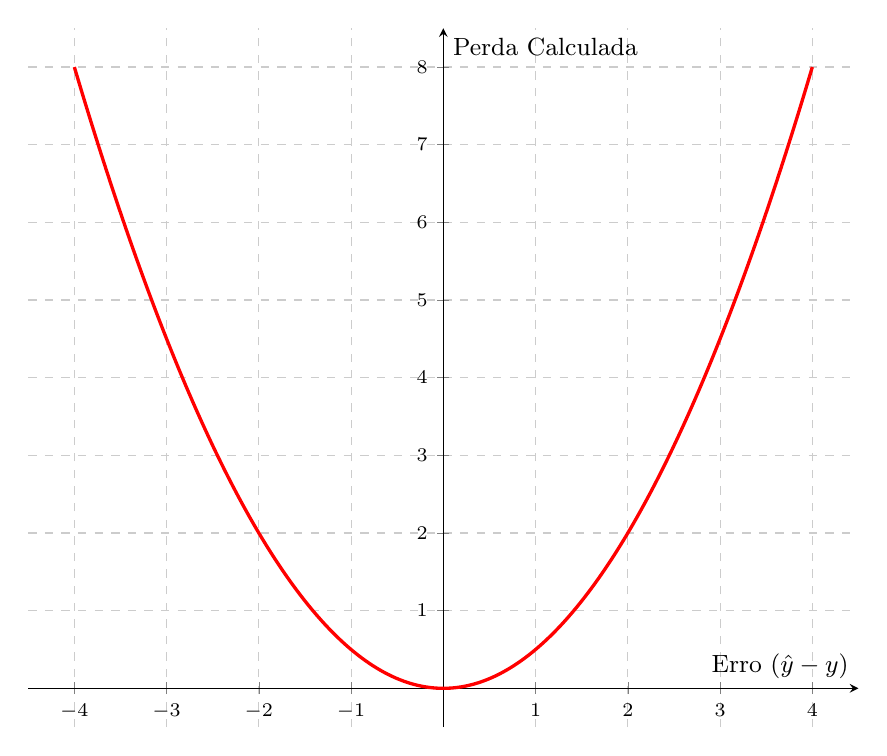
\begin{tikzpicture}
            \def\delta{4.0} % Delta grande
            \begin{axis}[
                xlabel={Erro ($\hat{y} - y$)},
                ylabel={Perda Calculada},
                axis lines=middle,
                grid=major,
                grid style={dashed, gray!40},
                xmin=-4.5, xmax=4.5,
                ymin=-0.5, ymax=8.5,
                legend pos=north west,
                width=\textwidth,
                label style={font=\small},
                tick label style={font=\scriptsize},
                title style={font=\bfseries, yshift=-5pt},
            ]
                % Função Huber Loss
                \addplot[
                    domain=-4:4, 
                    samples=201, 
                    color=red, 
                    very thick
                ] {(abs(x) <= \delta) ? (0.5*x^2) : (\delta*(abs(x) - 0.5*\delta))};

            \end{axis}
        \end{tikzpicture}
        \caption{Perda Huber com $\delta = 4.0$.}
        \label{fig:huber-comparacoes-mse}
    \end{subfigure}
    
    \caption{Comparação da Perda de Huber com diferentes valores de $\delta$.}
    \label{fig:huber-delta-comparacoes}
    \fonte{O autor (2025).}
\end{figure}

Assim, nota-se que ao utilizar a perda de Huber em um problema de regressão, é nítido que o grau de complexidade do problema pode aumentar, pois haverá mais um hiperparâmetro para ser otimizado de forma manual. Isso pode não ser ideal para cenários em que já existem muitos hiperparâmetros. Para isso, \textcite{LossesArticle} explicam que essa função é comumumente utilizada em problemas de gressão robusta, como em regressões lineares e em \textit{time series forecasting}, em que \textit{outliers} e ruído podem estar presentes.

\medskip
\begin{center}
 * * *
\end{center}
\medskip

\textbf{Algumas Apliações da Perda de Huber em Problemas de Regressão}
\vspace{1em}

\begin{itemize}
    \item \textbf{Aplicação 1 (Área):}
    \item \textbf{Aplicação 2 (Área):}
    \item \textbf{Aplicação 3 (Área):}
    \item \textbf{Aplicação 4 (Área):}
\end{itemize}

\medskip
\begin{center}
 * * *
\end{center}
\medskip

Com isso, foi possível ver que a perda de Huber é uma excelente alternativa para os casos em que deseja-se controlar os pontos em que o cálculo da perda deve atuar de forma severa (usando termos quadráticos, semelhante a perda L2) e a partir de quis casos esse cálculo pode ser menos punitivo (usando termos lineares, semelhante a perda L1). Contudo, foi visto que ela tem um problema, os pontos em que essas funções se juntam gera uma descontinuidade, atrabalhando a derivação dessas funções. Para resolver esse problema da descontinuidade, pode ser utilizada como alternativa a perda Log-Cosh, a qual será vista em seguida.

\subsection{Perda Log-Cosh}

A perda Log-Cosh é uma função de perda que vem ganhando popularidade entre os desenvolvedores, em \textit{Statistical Properties of the log-cosh Loss Function Used in Machine Learning}, \textcite{StatisticalPropetiesLogCosh} explicam que ela aparece em cenários de autoencoders variacionais, detecção de câncer, algortimos de aprendizado baseados em árvores (como o XGBoost) e também em regressão quantílica (\textit{quantile regression}).

Com relação a sua fórmula, é possível vê-la na Equação \ref{eq:log-cosh-loss}. Note que ela não adiciona nenhuma função nova, ela apenas faz a aplicação da função logaritmo que recebe como parâmetro de entrada a função cosseno hiperbólica. Essa combinação geram uma séries de propriedades interessantes, as quais serão discutidas depois ne analisar o seu gráfico.

\begin{equacaodestaque}{Perda Log-Cosh (\textit{Log-Cosh Loss})}
    \Loss_{\text{Log-Cosh}} = \sum_{j=1}^{N} \log(\cosh(y_j - \hat{y}_j))
    \label{eq:log-cosh-loss}
\end{equacaodestaque}

Já com relação ao gráfico dessa função, ele está presente na Figura \ref{fig:log-cosh-loss}. Note que a perda log-cosh atua de forma parecida com a perda de huber. Para valores em que a diferença da saída do modelo e o rôtulo real ($y_j - \hat{y}_j$) é pequena, ela tem um comportamento que lembra ao de uma função quadrática (como o \textit{MSE}). Além disso, conforme o resultado dessa diferença de valores aumenta, a perda log-cosh passa a assumir um comportamento parecido com o de uma função linear (como o \textit{MAE}). Em testes realizados por \textcite{StatisticalPropetiesLogCosh}, a perda log-cosh foi comparada com a perda de Huber, e foi verificado que as estimativas dessas funcoes bem como os erros padroes apresentam resultados similares. Com isso, ela pode ser uma alternativa a ser considerada caso sejam encontrados problemas ao utilizar a \textit{Huber Loss}, mas ainda é desejável manter a variação no cálculo do erro do modelo.

\begin{figure}[h!]
    \centering % Centraliza a figura na página

    % --- SUBFIGURA (a): Gráfico 2D da Log-Cosh Loss ---
    \begin{subfigure}[b]{0.48\textwidth}
        \centering
        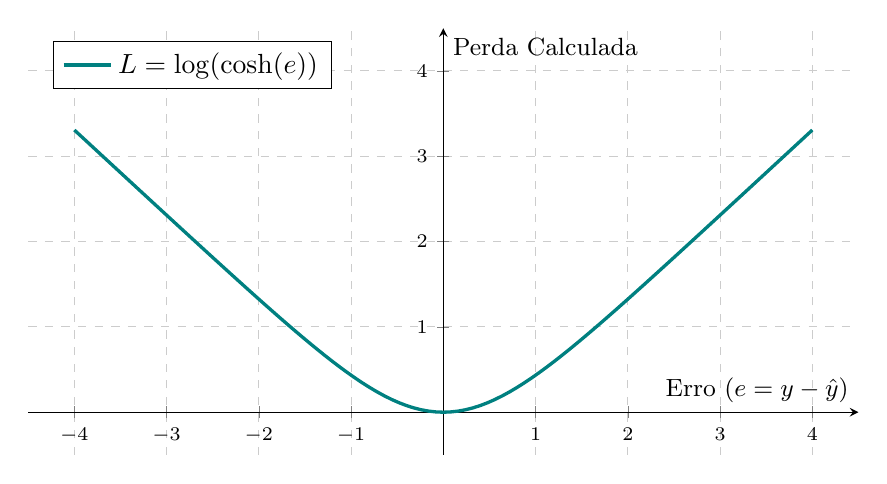
\begin{tikzpicture}
            \begin{axis}[
                % Dimensões ajustadas para caber lado a lado
                width=\linewidth,  
                height=7cm,
                xlabel={Erro ($e = y - \hat{y}$)},
                ylabel={Perda Calculada},
                axis lines=middle,
                grid=major,
                grid style={dashed, gray!40},
                xmin=-4.5, xmax=4.5,        % Limites do seu gráfico
                ymin=-0.5, ymax=4.5,         % Limites do seu gráfico
                legend pos=north west,
                title style={font=\bfseries\small},
                label style={font=\small},
                tick label style={font=\scriptsize}
            ]
                % Gráfico da função ln(cosh(x))
                \addplot[
                    domain=-4:4, 
                    samples=101,
                    color=teal, 
                    very thick
                ] {ln(cosh(x))};
                
                \addlegendentry{$L = \log(\cosh(e))$}
            \end{axis}
        \end{tikzpicture}
        \caption{Representação gráfica em duas dimensões.} % Legenda da subfigura
        \label{fig:log-cosh-2d}
    \end{subfigure}
    \hfill % Adiciona espaço horizontal flexível entre as subfiguras
    % --- SUBFIGURA (b): Gráfico 3D da Log-Cosh Loss ---
    \begin{subfigure}[b]{0.48\textwidth}
        \centering
        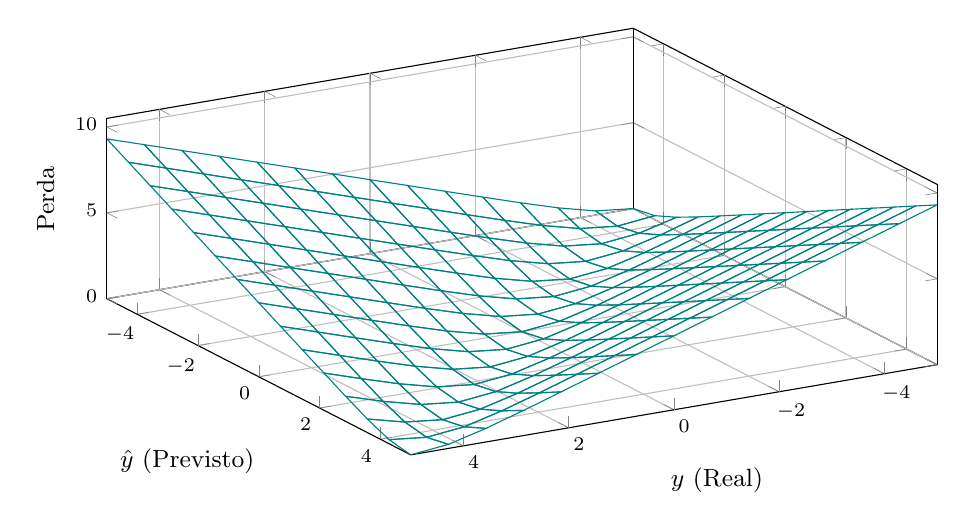
\begin{tikzpicture}
            \begin{axis}[
                % Dimensões consistentes com o gráfico (a)
                width=\linewidth,
                height=7cm,
                xlabel={$y$ (Real)},
                ylabel={$\hat{y}$ (Previsto)},
                zlabel={Perda},
                grid=major,
                view={150}{45}, % Mesmo ângulo de visão do seu template
                zmin=0, zmax=10.5, % Limite Z ajustado para Log-Cosh com domínio -5:5
                title style={font=\bfseries\small},
                label style={font=\small},
                tick label style={font=\scriptsize}
            ]
                % Gráfico da superfície da Log-Cosh Loss
                \addplot3[
                    mesh,           
                    color=teal,     % Cor consistente com o gráfico 2D
                    shader=interp,  
                    domain=-5:5,    % Mesmo domínio do seu template
                    domain y=-5:5,  % Mesmo domínio do seu template
                    samples=15      % Mesma resolução da malha
                ] { ln(cosh(x - y)) }; % A função Log-Cosh 3D
            \end{axis}
        \end{tikzpicture}
        \caption{Representação gráfica em três dimensões.} % Legenda da subfigura
        \label{fig:log-cosh-3d}
    \end{subfigure}

    % --- Legenda e Fonte da Figura Principal ---
    \caption{Visualizações da função de perda Log-Cosh (\textit{Log-Cosh Loss}) em duas e em três dimensões.}
    \label{fig:log-cosh-loss} % Rótulo principal do seu gráfico
    \fonte{O autor (2025).}
\end{figure}

\medskip
\begin{center}
 * * *
\end{center}
\medskip

\textbf{Características da Perda Log-Cosh}
\vspace{1em}

Com relação as suas propriedades é possível discutir algumas a seguir:

\begin{itemize}
    \item \textbf{Convexa:} É possível ver pelo gráfico da Figura \ref{fig:log-cosh-loss} que ela é uma função convexa, apresentando um formato característico de funil, além de possuír um único ponto de mínimo global. Mas note que não é possível garantir essa propriedade em cenários em que ela está sendo aplicada em modelos de redes neurais densas, devido as transformações não-lineares que ocorrem.
    \item \textbf{Robustez para \textit{outliers}:} Assim como a perda de Huber e o erro absoluto médio, a perda log-cosh não pune de forma agressiva os erros cometidos pelo modelo ao ser treinado. Isso garante que essa função possa ser aplicada em cenários em que os dados possuem muitos \textit{outliers} sem afetar drasticamente o treinamento do modelo.
    \item \textbf{Continuidade e diferenciabilidade:} Diferente de a perda de Huber, que possui pontos de descontuidade na ligação da função linear com a quadrática, a perda log-cosh consegue ser contínua em todos os seus pontos. Além disso, isso também é uma vantagem sobre o erro absoluto médio, pois este também apresenta um ponto de descontinuidade em 0, o qual precisa do cálculo do subgradiente para garantir o aprendizado dos modelos que fazem uso de otimizadores baseados em gradiente. Dessa forma, além de ser contínua, a perda log-cosh pode ser derivada em todos os seus pontos, algo útil caso esteja sendo usados otimizadores que atuam como o método do gradiente.
\end{itemize}

\medskip
\begin{center}
 * * *
\end{center}
\medskip

Visto essas diferentes propriedades dessa função, cabe agora analisar a sua derivada, a qual será útil para a retropropagação e consequentemente o aprendizado do modelo. Para isso, ela pode ser vista na Equação \ref{eq:log-cosh-derivada}. Perceba que a derivada da perda log-cosh envolve o cálculo da tangente hiperbólica, que coincidementemente, também é utilizada em aprendizado de máquina como uma função de ativação, tendo como objetivo introduzir a não-liearidade para as saídas de uma camada densa.

\begin{equacaodestaque}{Derivada da Perda Log-Cosh}
    \frac{\partial \Loss_{\text{Log-Cosh}}}{\partial \hat{y}_j} = \tanh(\hat{y}_j - y_j)
    \label{eq:log-cosh-derivada}
\end{equacaodestaque}

Tendo a fórmula da sua derivada, o próximo passo é analisar o seu gráfico, o qual está representado na Figura \ref{eq:log-cosh-derivada}. Caso você leitor tenha lido o Capítulo \ref{cap:ativacao-sigmoidais}, você não verá nada novo aqui, é apenas o gráfico característico em formato de "S" que as funções sigmoidais possuem. Um ponto interessante a ser destacado ao analisar o gráfico é que as saídas dessa função serão em um intervalo $[-1, 1]$, o que podem fazer com que o sinal do gradiente fique alternando, garantindo uma convergência mais rápida em alguns casos.

\begin{figure}[h!]
    \centering % Centraliza a figura na página

    % --- SUBFIGURA (a): Gráfico 2D da Derivada da Log-Cosh ---
    \begin{subfigure}[b]{0.48\textwidth}
        \centering
        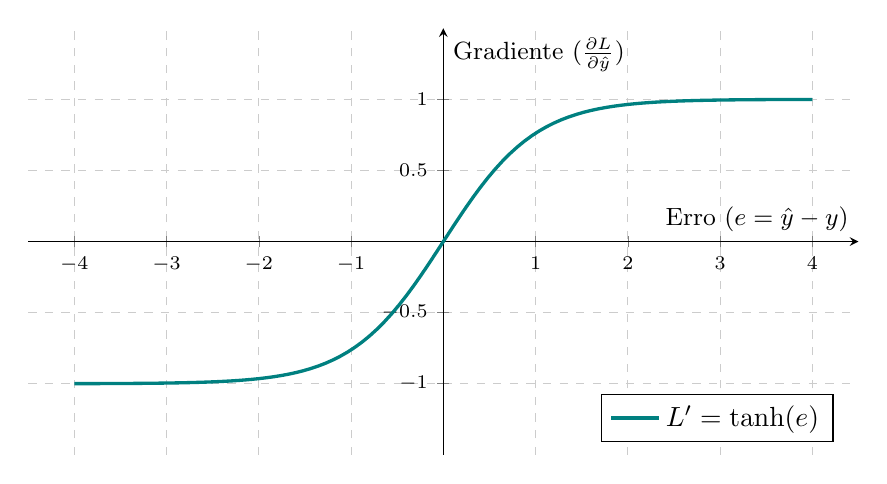
\begin{tikzpicture}
            \begin{axis}[
                % Dimensões ajustadas para caber lado a lado
                width=\linewidth,  
                height=7cm,
                xlabel={Erro ($e = \hat{y} - y$)},
                ylabel={Gradiente ($\frac{\partial L}{\partial \hat{y}}$)},
                axis lines=middle,
                grid=major,
                grid style={dashed, gray!40},
                xmin=-4.5, xmax=4.5,        % Limites do seu gráfico
                ymin=-1.5, ymax=1.5,         % Limites do seu gráfico
                ytick={-1, -0.5, 0, 0.5, 1}, % Marcas no eixo y
                legend pos=south east,
                title style={font=\bfseries\small},
                label style={font=\small},
                tick label style={font=\scriptsize}
            ]
                % Gráfico da função tanh(x)
                \addplot[
                    domain=-4:4, 
                    samples=101,
                    color=teal, 
                    very thick
                ] {tanh(x)};
                
                \addlegendentry{$L' = \tanh(e)$}
            \end{axis}
        \end{tikzpicture}
        \caption{Visão 2D (Gradiente vs. Erro).} % Legenda da subfigura
        \label{fig:log-cosh-derivada-2d}
    \end{subfigure}
    \hfill % Adiciona espaço horizontal flexível entre as subfiguras
    % --- SUBFIGURA (b): Gráfico 3D da Derivada da Log-Cosh ---
    \begin{subfigure}[b]{0.48\textwidth}
        \centering
        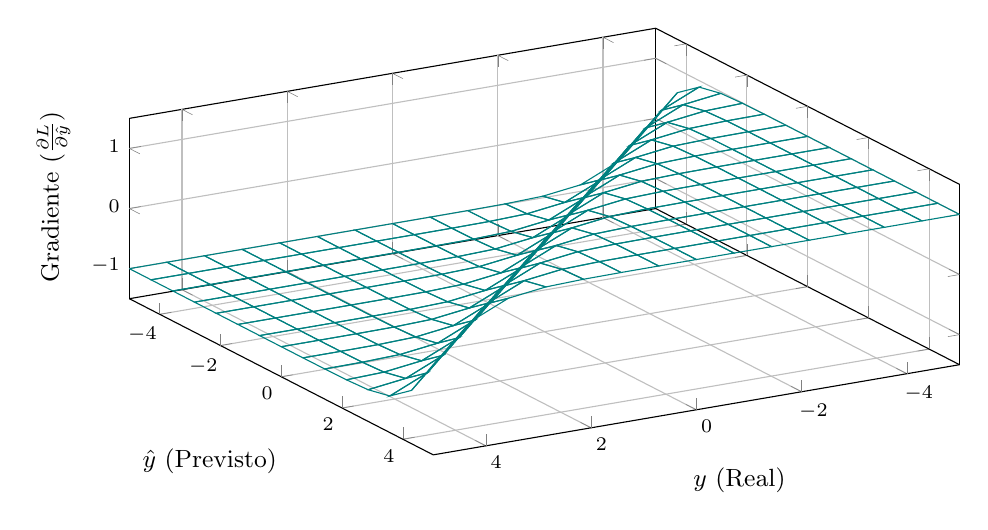
\begin{tikzpicture}
            \begin{axis}[
                % Dimensões consistentes com o gráfico (a)
                width=\linewidth,
                height=7cm,
                xlabel={$y$ (Real)},
                ylabel={$\hat{y}$ (Previsto)},
                zlabel={Gradiente ($\frac{\partial L}{\partial \hat{y}}$)},
                grid=major,
                view={150}{45}, % Mesmo ângulo de visão do seu template
                zmin=-1.5, zmax=1.5, % Espelha o eixo Y do gráfico 2D
                ztick={-1, 0, 1}, % Consistente com o 2D
                title style={font=\bfseries\small},
                label style={font=\small},
                tick label style={font=\scriptsize}
            ]
                % Gráfico da superfície do gradiente: tanh(y_hat - y)
                \addplot3[
                    mesh,           
                    color=teal,     % Cor consistente com o gráfico 2D
                    shader=interp,  
                    domain=-5:5,    % Mesmo domínio do seu template
                    domain y=-5:5,  % Mesmo domínio do seu template
                    samples=15      % Mesma resolução da malha
                ] { tanh(y - x) }; % A função da derivada: tanh(y_previsto - y_real)
            \end{axis}
        \end{tikzpicture}
        \caption{Superfície 3D completa.} % Legenda da subfigura
        \label{fig:log-cosh-derivada-3d}
    \end{subfigure}

    % --- Legenda e Fonte da Figura Principal ---
    \caption{Visualizações da derivada (gradiente) da função de perda Log-Cosh.}
    \label{fig:log-cosh-derivada} % Rótulo principal do seu gráfico
    \fonte{O autor (2025).}
\end{figure}

\medskip
\begin{center}
 * * *
\end{center}
\medskip

\textbf{Algumas Aplicações da Perda Log-Cosh em Problemas de Regressão}
\vspace{1em}

\begin{itemize}
    \item \textbf{Aplicação 1 (Área):}
    \item \textbf{Aplicação 2 (Área):}
    \item \textbf{Aplicação 3 (Área):}
    \item \textbf{Aplicação 4 (Área):}
\end{itemize}

\medskip
\begin{center}
 * * *
\end{center}
\medskip

Vistas essas quatro funções: O erro quadrático médio (\textit{MSE}), o erro absoluto médio (\textit{MAE}), a perda de Huber e a perda log-cosh. Já é possível resolver a grande maioria dos problemas de regressão em aprendizado de máquina. Contudo, existem problemas que vão além dessas perdas, precisando de funções mais específicas para garantir uma melhor avaliação do erro e a partir dele, saber atualizar o gradiente e com isso o modelo aprender de fato.

Para isso, as próximas seções buscam explorar diferentes cenários em que as funções de perda para regressão vistas até agora não são a melhor escolha. Assim, serão exploradas mais três secões, a primeira focada no erro relativo, a segunda focada em funções de erro que não calculam a média dos diversos erros, e a última para casos em são utilizas distribuições específicas para os valores.

\section{Lidando com a Escala: Foco no Erro Relativo}

As funções de perda vistas até agora possuem um detalhe em comum: todas lidam com o erro de fazendo um cálculo absoluto. Para entender melhor essa frase é possível ilustrar isso com um exemplo. Considere que existem duas situações que está sendo previsto os valores de imóveis:

\begin{itemize}
    \item Cenário A: O modelo previu que uma casa vale 50.000 R\$, equanto no rótulo está que ela vale 10.000 R\$;
    \item Cenário B: O modelo previu que uma casa vale 950.000 R\$, equanto no rótulo está que ela vale 1.000.000 R\$.
\end{itemize}

Para fazer o trabalho dessa regressão foi utilizada a função de perda erro quadrático médio. Note que essa função calcula primeiro a diferença entre o valor previsto pelo modelo e o valor apresentado no rótulo. Com isso, essa diferença será a mesma para esses dois cenários, 50.000 R\$.

Essa é uma forma de analisar o problema. Mas também pode ser visto de forma relativa, veja que o modelo do cenário A previu que a casa vale apenas a metade do seu valor real, ele fez uma previsão subestimada. Por outro lado, o modelo do cenário B foi mais realista, ele sabe que a casa possui um valor alto, contudo, ainda sim ficou uma distância do valor real. 

O erro quadrático médio, e as outras três funções de perda vistas até agora tratam os erros dos cenários A e B como iguais. Mas e se você estivesse em uma situação em que o modelo subestimar os valores dos rôtulos seja considerada muito negativa, e por isso deve ser evitada?

Aí você precisaria de funções de perda que lidassem com o erro relativo das previsões do modelo. Para isso, esse capítulo busca explicar três funções de perda para serem utilizadas nesse cenário. O erro quadrático médio logarítico, que possui uma tendência de penalizar mais as subestimação. O erro percentual absoluto médio, que funciona de forma aposta o \textit{MSLE}, penalizando mais a superestimação, porém com um problema de descontinuidade que pode fazer com que o cálculo da métrica "exploda". E por fim, será visto o erro percentual absoluto médio simétrico, o qual busca corrigir o problema da descontinuidade da sua variante original.

\subsection{Erro Quadrático Médio Logarítmico (MSLE)}

A primeira função a ser vista nessa nova categoria é o erro quadrático médio logarítimico, também chamado de \textit{Mean Squared Logarithmic Error} (\textit{MSLE}). A sua fórmula é dada pela Equação \ref{eq:msle-loss}. Perceba que diferente das funções vistas até agora, ela faz o cálculo do logaritmo natural dos valores reais ($y_j$) e dos valores previstos pelo modelo ($\hat{y}_j$). Além disso, um ponto que vale a pena ser destacado é com relação ao valor de 1 que é somado aos valores antes do cálculo do logaritmo. Isso ocorre para evitar com que esse resultado possa ser negativo ou zero, gerando uma indeterminação ao calcular o logaritimo.

\begin{equacaodestaque}{Erro Quadrático Médio Logarítmico (\textit{MSLE})}
    \Loss_{\text{MSLE}} = \frac{1}{N} \sum_{j=1}^{N} (\log(y_j + 1) - \log(\hat{y}_j + 1))^2
    \label{eq:msle-loss}
\end{equacaodestaque}

Com relação ao seu gráfico, ele pode visto na Figura \ref{fig:msle-loss}. Na Figura \ref{fig:msle-2d}, a esquerda, está a visão em duas dimensões dessa função, enquanto na Figura \ref{fig:msle-3d}, a direita, está a visão em três dimensões. Perceba que a adição do logaritmo para essa função traz alguns benefícios como a continuidade em seus pontos além de garantir uma superfície suave e diferenciável. Contudo, a pricipal característica dessa função é que ela é uma função assimétrica com relação ao eixo $y$ e por consequência, ela apresenta uma tendência de penalizar mais as subestimações feitas pelo modelo.

\begin{figure}[h!]
    \centering % Centraliza a figura na página

    % --- SUBFIGURA (a): Gráfico 2D da MSLE (Corte em y=10) ---
    \begin{subfigure}[b]{0.48\textwidth}
        \centering
        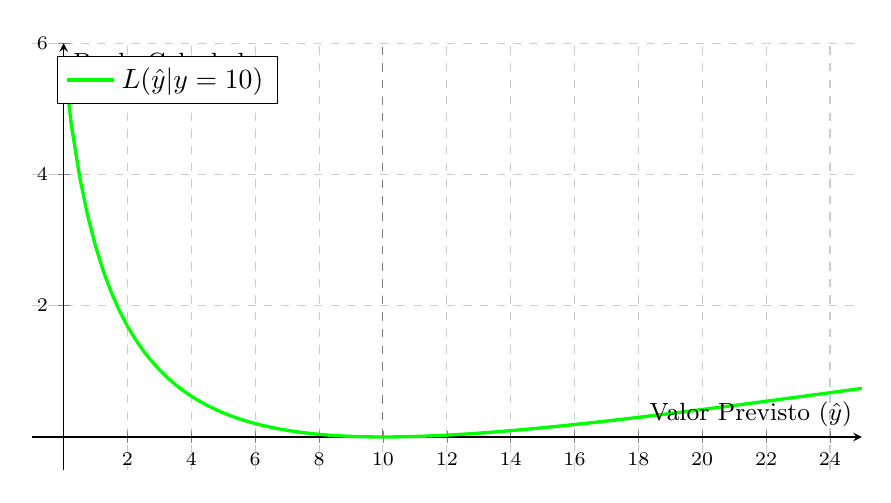
\begin{tikzpicture}
            \begin{axis}[
                % Dimensões ajustadas para caber lado a lado
                width=\linewidth,  
                height=7cm,
                xlabel={Valor Previsto ($\hat{y}$)},
                ylabel={Perda Calculada},
                axis lines=middle,
                grid=major,
                grid style={dashed, gray!40},
                xmin=-1, xmax=25,        % Limites do seu gráfico
                ymin=-0.5, ymax=6,         % Limites do seu gráfico
                legend pos=north west,
                title style={font=\bfseries\small},
                label style={font=\small},
                tick label style={font=\scriptsize}
            ]
                % Gráfico da função (ln(11) - ln(x+1))^2
                \addplot[
                    domain=0:25, 
                    samples=101,
                    color=green, 
                    very thick
                ] {(ln(10+1) - ln(x+1))^2};
                
                \addlegendentry{$L(\hat{y} | y=10)$}

                % Linha vertical para marcar o valor real
                \draw[dashed, gray] (axis cs:10, 0) -- (axis cs:10, 6);
                \node[above, gray!80, font=\tiny] at (axis cs:10, 6) {Valor Real ($y=10$)};
            \end{axis}
        \end{tikzpicture}
        \caption{Visão 2D (corte em $y=10$).} % Legenda da subfigura
        \label{fig:msle-2d}
    \end{subfigure}
    \hfill % Adiciona espaço horizontal flexível entre as subfiguras
    % --- SUBFIGURA (b): Gráfico 3D da MSLE ---
    \begin{subfigure}[b]{0.48\textwidth}
        \centering
        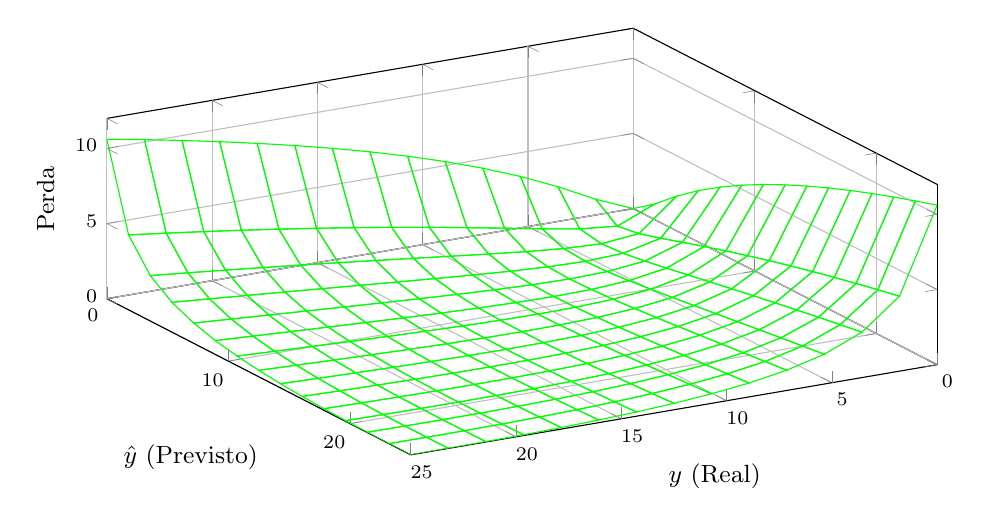
\begin{tikzpicture}
            \begin{axis}[
                % Dimensões consistentes com o gráfico (a)
                width=\linewidth,
                height=7cm,
                xlabel={$y$ (Real)},
                ylabel={$\hat{y}$ (Previsto)},
                zlabel={Perda},
                grid=major,
                view={150}{45}, % Mesmo ângulo de visão do seu template
                zmin=0, zmax=12, % Ajustado para (ln(26)-ln(1))^2
                title style={font=\bfseries\small},
                label style={font=\small},
                tick label style={font=\scriptsize}
            ]
                % Gráfico da superfície da MSLE
                \addplot3[
                    mesh,           
                    color=green,    % Cor consistente com o gráfico 2D
                    shader=interp,  
                    domain=0:25,    % Domínio > -1 (usando 0:25)
                    domain y=0:25,  % Domínio > -1 (usando 0:25)
                    samples=15      % Mesma resolução da malha
                ] { (ln(x+1) - ln(y+1))^2 }; % A função MSLE 3D
            \end{axis}
        \end{tikzpicture}
        \caption{Superfície 3D completa.} % Legenda da subfigura
        \label{fig:msle-3d}
    \end{subfigure}

    % --- Legenda e Fonte da Figura Principal ---
    \caption{Visualizações da função de perda MSLE (\textit{Mean Squared Logarithmic Error}).}
    \label{fig:msle-loss} % Rótulo principal do seu gráfico
    \fonte{O autor (2025).}
\end{figure}

\medskip
\begin{center}
 * * *
\end{center}
\medskip

\textbf{Características do Erro Quadrático Médio Logarítmico}
\vspace{1em}

Conhecendo a fórmula dessa função e suas representações gráficas, cabe agora discutir algumas das características dessa função:

\begin{itemize}
    \item \textbf{Tendência de penalizar subestimações:} Como pode ser visto nos gráficos da Figura \ref{fig:msle-loss}, a função \textit{MSLE} não forma uma curva convexa simétrica verticalmente, perceba que conforme os valores vão diminuindo, a perda aumenta consideravelmente. Enquanto isso, conforme os valores aumentam, a perda também aumenta, mas não de forma tão agressiva quanto no sentido inverso. Isso significa que quanto menor for a diferença entre o valor previsto $\hat{y}_j$ e o valor real $y_j$, existe uma tendência de que a perda será maior.
    \item \textbf{Continuidade e Diferencibilidade:} Ainda com relação aos seus gráficos é possível analisar a continuidade dessa função. Note que ela não apresenta nenhum ponto "problema" que poderia afetar o cálculo das derivadas e com isso atrabalhar o fluxo do gradiente. Além disso, o uso dos logaritmos para essa função permite que suas curvas sejam suaves, o que também ajuda na sua continuidade.
\end{itemize}

\medskip
\begin{center}
 * * *
\end{center}
\medskip

\begin{equacaodestaque}{Derivada do Erro Quadrático Médio Logarítmico (\textit{MSLE})}
    \frac{\partial \Loss_{\text{MSLE}}}{\partial \hat{y}_j} = - \frac{2}{N} \cdot \frac{\log(y_j + 1) - \log(\hat{y}_j + 1)}{\hat{y}_j + 1}
    \label{eq:msle-derivada}
\end{equacaodestaque}

\begin{figure}[h!]
    \centering % Centraliza a figura na página

    % --- SUBFIGURA (a): Gráfico 2D da Derivada da MSLE (Corte em y=10) ---
    \begin{subfigure}[b]{0.48\textwidth}
        \centering
        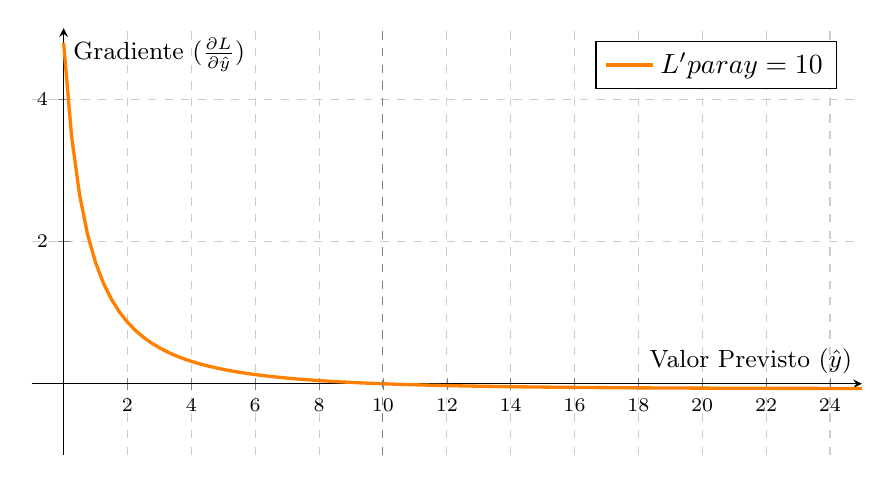
\begin{tikzpicture}
            \begin{axis}[
                % Dimensões ajustadas para caber lado a lado
                width=\linewidth,  
                height=7cm,
                xlabel={Valor Previsto ($\hat{y}$)},
                ylabel={Gradiente ($\frac{\partial L}{\partial \hat{y}}$)},
                axis lines=middle,
                grid=major,
                grid style={dashed, gray!40},
                xmin=-1, xmax=25,        % Limites do seu gráfico
                ymin=-1, ymax=5,         % Limites do seu gráfico
                legend pos=north east,
                title style={font=\bfseries\small},
                label style={font=\small},
                tick label style={font=\scriptsize}
            ]
                % Gráfico da derivada (fórmula corrigida para corresponder aos eixos)
                \addplot[
                    domain=0:25, 
                    samples=101,
                    color=orange, 
                    very thick
                ] {2 * (ln(10+1) - ln(x+1)) / (x+1)}; % Corrigido (removido o -)
                
                \addlegendentry{$L' \text{ para } y=10$}

                % Linha vertical para marcar o valor real
                \draw[dashed, gray] (axis cs:10, -1) -- (axis cs:10, 5);
                \node[above, gray!80, font=\tiny] at (axis cs:10, 5) {Valor Real};
            \end{axis}
        \end{tikzpicture}
        \caption{Visão 2D (corte em $y=10$).} % Legenda da subfigura
        \label{fig:msle-derivada-2d}
    \end{subfigure}
    \hfill % Adiciona espaço horizontal flexível entre as subfiguras
    % --- SUBFIGURA (b): Gráfico 3D da Derivada da MSLE ---
    \begin{subfigure}[b]{0.48\textwidth}
        \centering
        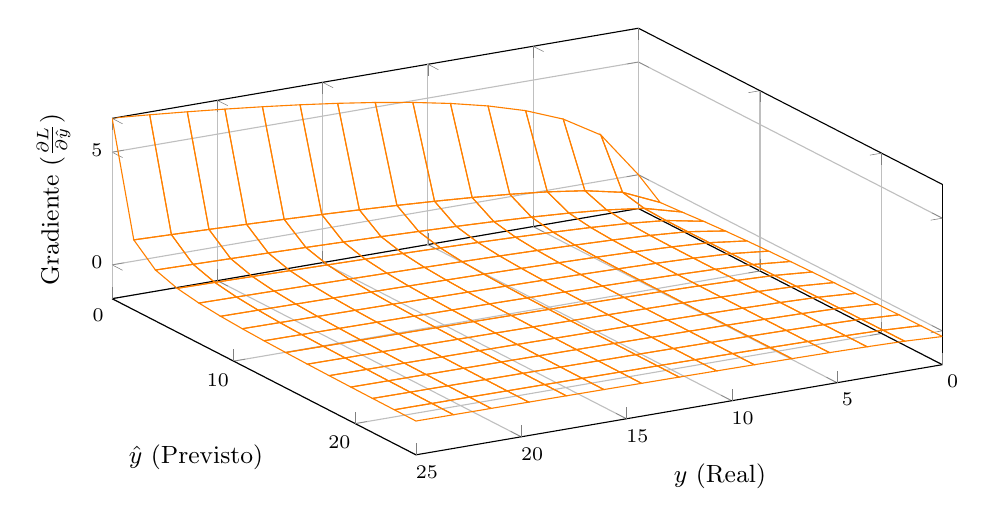
\begin{tikzpicture}
            \begin{axis}[
                % Dimensões consistentes com o gráfico (a)
                width=\linewidth,
                height=7cm,
                xlabel={$y$ (Real)},
                ylabel={$\hat{y}$ (Previsto)},
                zlabel={Gradiente ($\frac{\partial L}{\partial \hat{y}}$)},
                grid=major,
                view={150}{45}, % Mesmo ângulo de visão do seu template
                zmin=-1.5, zmax=6.5, % Ajustado para o pico do gradiente
                title style={font=\bfseries\small},
                label style={font=\small},
                tick label style={font=\scriptsize}
            ]
                % Gráfico da superfície da derivada da MSLE (fórmula corrigida)
                \addplot3[
                    mesh,           
                    color=orange,   % Cor consistente com o gráfico 2D
                    shader=interp,  
                    domain=0:25,    % Domínio de x (y_real)
                    domain y=0:25,  % Domínio de y (y_previsto)
                    samples=15      % Mesma resolução da malha
                ] { 2 * (ln(x+1) - ln(y+1)) / (y+1) }; % L' = 2(log(y+1)-log(y_hat+1))/(y_hat+1)
            \end{axis}
        \end{tikzpicture}
        \caption{Superfície 3D completa.} % Legenda da subfigura
        \label{fig:msle-derivada-3d}
    \end{subfigure}

    % --- Legenda e Fonte da Figura Principal ---
    \caption{Visualizações da derivada (gradiente) da função de perda MSLE.}
    \label{fig:msle-derivada} % Rótulo principal do seu gráfico
    \fonte{O autor (2025).}
\end{figure}

\medskip
\begin{center}
 * * *
\end{center}
\medskip

\textbf{Algumas Aplicações do Erro Quadrático Logarítimico Médio em Problemas de Regressão}
\vspace{1em}

\begin{itemize}
    \item \textbf{Aplicação 1 (Área):}
    \item \textbf{Aplicação 2 (Área):}
    \item \textbf{Aplicação 3 (Área):}
    \item \textbf{Aplicação 4 (Área):}
\end{itemize}

\subsection{Erro Percentual Absoluto Médio (MAPE)}

\begin{equacaodestaque}{Erro Percentual Absoluto Médio (\textit{MAPE})}
    \Loss_{\text{MAPE}} = \frac{1}{N} \sum_{j=1}^{N} \left| \frac{y_j - \hat{y}_j}{y_j} \right|
    \label{eq:mape-loss}
\end{equacaodestaque}

\begin{figure}[h!]
    \centering % Centraliza a figura na página

    % --- SUBFIGURA (a): Gráfico 2D da MAPE (Corte em y=10) ---
    \begin{subfigure}[b]{0.48\textwidth}
        \centering
        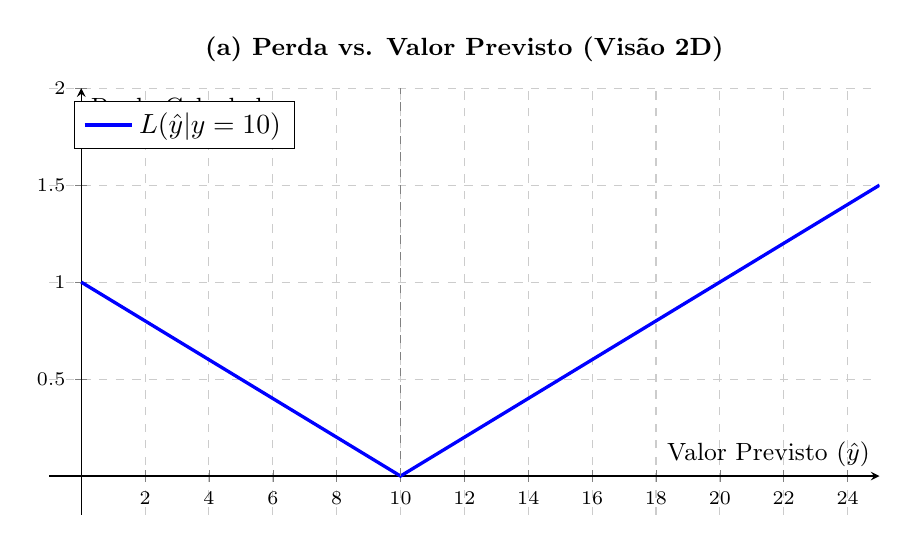
\begin{tikzpicture}
            \begin{axis}[
                % Dimensões ajustadas para caber lado a lado
                width=\linewidth,  
                height=7cm,
                title={(a) Perda vs. Valor Previsto (Visão 2D)},
                xlabel={Valor Previsto ($\hat{y}$)},
                ylabel={Perda Calculada},
                axis lines=middle,
                grid=major,
                grid style={dashed, gray!40},
                xmin=-1, xmax=25,        % Limites do seu gráfico
                ymin=-0.2, ymax=2,         % Limites do seu gráfico
                legend pos=north west,
                title style={font=\bfseries\small},
                label style={font=\small},
                tick label style={font=\scriptsize}
            ]
                % Gráfico da função abs((10 - x) / 10)
                \addplot[
                    domain=0:25, 
                    samples=101,
                    color=blue, 
                    very thick
                ] {abs((10 - x) / 10)};
                
                \addlegendentry{$L(\hat{y} | y=10)$}

                % Linha vertical para marcar o valor real
                \draw[dashed, gray] (axis cs:10, 0) -- (axis cs:10, 2);
                \node[above, gray!80, font=\tiny] at (axis cs:10, 2) {Valor Real ($y=10$)};
            \end{axis}
        \end{tikzpicture}
        \caption{Visão 2D (corte em $y=10$).} % Legenda da subfigura
        \label{fig:mape-2d}
    \end{subfigure}
    \hfill % Adiciona espaço horizontal flexível entre as subfiguras
    % --- SUBFIGURA (b): Gráfico 3D da MAPE ---
    \begin{subfigure}[b]{0.48\textwidth}
        \centering
        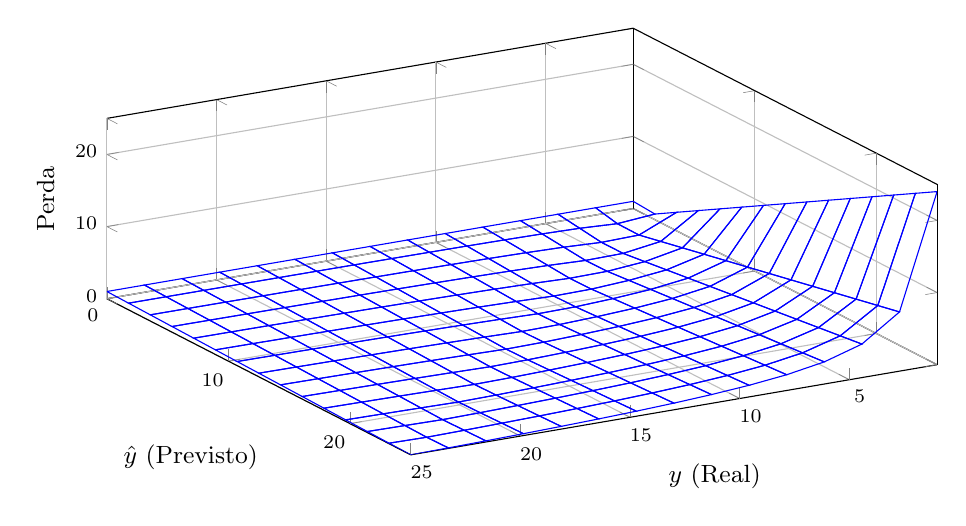
\begin{tikzpicture}
            \begin{axis}[
                % Dimensões consistentes com o gráfico (a)
                width=\linewidth,
                height=7cm,
                xlabel={$y$ (Real)},
                ylabel={$\hat{y}$ (Previsto)},
                zlabel={Perda},
                grid=major,
                view={150}{45}, % Mesmo ângulo de visão do seu template
                zmin=0, zmax=25, % Ajustado para o domínio
                title style={font=\bfseries\small},
                label style={font=\small},
                tick label style={font=\scriptsize}
            ]
                % Gráfico da superfície da MAPE
                \addplot3[
                    mesh,           
                    color=blue,     % Cor consistente com o gráfico 2D
                    shader=interp,  
                    domain=1:25,    % Domínio de x (y_real) > 0 para evitar divisão por zero
                    domain y=0:25,  % Domínio de y (y_previsto)
                    samples=15      % Mesma resolução da malha
                ] { abs((x - y) / x) }; % A função MAPE 3D: L = |(y - y_hat) / y|
            \end{axis}
        \end{tikzpicture}
        \caption{Superfície 3D completa ($y>0$).} % Legenda da subfigura
        \label{fig:mape-3d}
    \end{subfigure}

    % --- Legenda e Fonte da Figura Principal ---
    \caption{Visualizações da função de perda MAPE (\textit{Mean Absolute Percentage Error}).}
    \label{fig:mape-loss} % Rótulo principal do seu gráfico
    \fonte{O autor (2025).}
\end{figure}

\medskip
\begin{center}
 * * *
\end{center}
\medskip

\textbf{Características do Erro Percentual Absoluto Médio}
\vspace{1em}

\begin{itemize}
    \item \textbf{Característica 1:}
    \item \textbf{Característica 2:}
    \item \textbf{Característica 3:}
\end{itemize}

\medskip
\begin{center}
 * * *
\end{center}
\medskip

\begin{equacaodestaque}{Derivada do Erro Percentual Absoluto Médio (\textit{MAPE})}
    \frac{\partial \Loss_{\text{MAPE}}}{\partial \hat{y}_j} = - \frac{1}{N} \cdot \frac{\text{sgn}(y_j - \hat{y}_j)}{y_j}
    \label{eq:mape-derivada}
\end{equacaodestaque}

\begin{figure}[h!]
    \centering % Centraliza a figura na página

    % --- SUBFIGURA (a): Gráfico 2D da Derivada da MAPE (Corte em y=10) ---
    \begin{subfigure}[b]{0.48\textwidth}
        \centering
        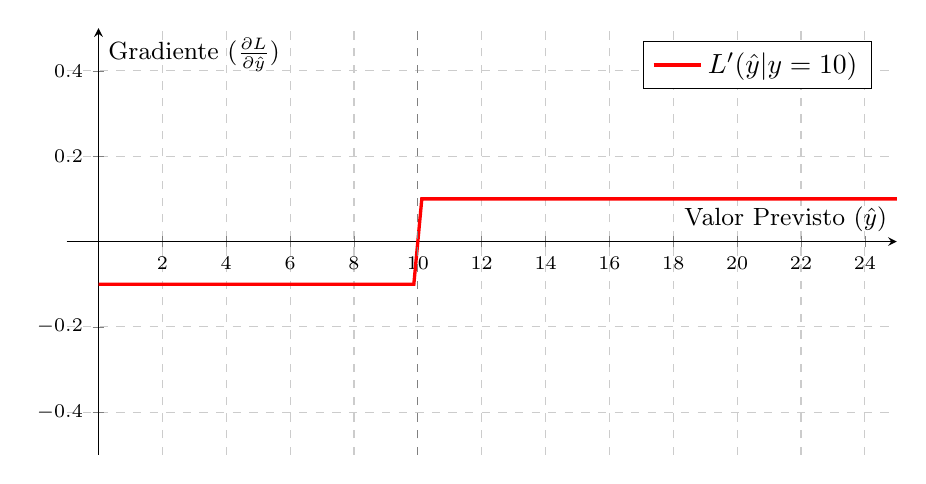
\begin{tikzpicture}
            \begin{axis}[
                % Dimensões ajustadas para caber lado a lado
                width=\linewidth,  
                height=7cm,
                xlabel={Valor Previsto ($\hat{y}$)},
                ylabel={Gradiente ($\frac{\partial L}{\partial \hat{y}}$)},
                axis lines=middle,
                grid=major,
                grid style={dashed, gray!40},
                xmin=-1, xmax=25,        % Limites do seu gráfico
                ymin=-0.5, ymax=0.5,         % Limites do seu gráfico
                legend pos=north east,
                title style={font=\bfseries\small},
                label style={font=\small},
                tick label style={font=\scriptsize},
                declare function={sgn(\x) = (\x > 0) - (\x < 0);} % Função Sinal
            ]
                % Gráfico da derivada
                \addplot[
                    domain=0:25, 
                    samples=201,
                    color=red, 
                    very thick
                ] {-sgn(10-x)/10};
                
                \addlegendentry{$L'(\hat{y} | y=10)$}

                % Linha vertical
                \draw[dashed, gray] (axis cs:10, -0.5) -- (axis cs:10, 0.5);
                \node[above, gray!80, font=\tiny] at (axis cs:10, 0.5) {Valor Real};
            \end{axis}
        \end{tikzpicture}
        \caption{Visão 2D (corte em $y=10$).} % Legenda da subfigura
        \label{fig:mape-derivada-2d}
    \end{subfigure}
    \hfill % Adiciona espaço horizontal flexível entre as subfiguras
    % --- SUBFIGURA (b): Gráfico 3D da Derivada da MAPE ---
    \begin{subfigure}[b]{0.48\textwidth}
        \centering
        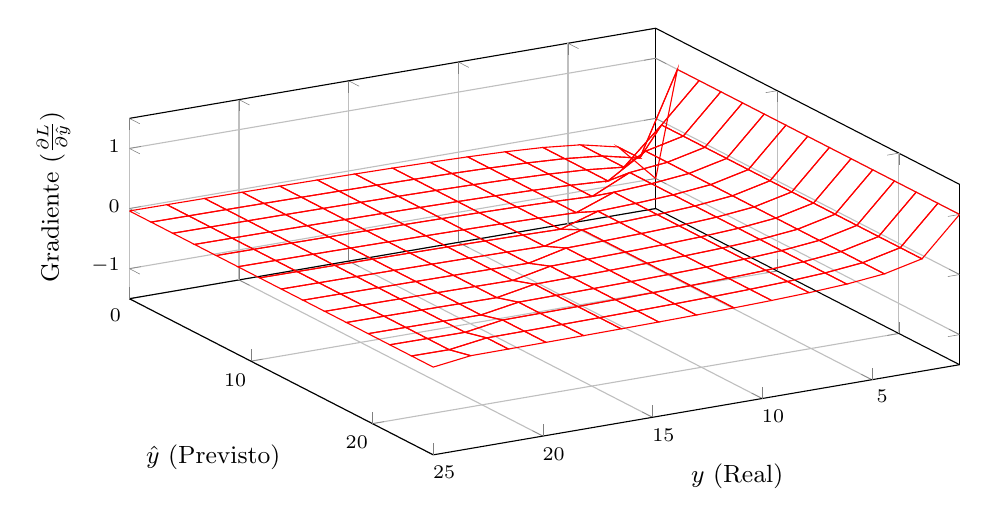
\begin{tikzpicture}
            \begin{axis}[
                % Dimensões consistentes com o gráfico (a)
                width=\linewidth,
                height=7cm,
                xlabel={$y$ (Real)},
                ylabel={$\hat{y}$ (Previsto)},
                zlabel={Gradiente ($\frac{\partial L}{\partial \hat{y}}$)},
                grid=major,
                view={150}{45}, % Mesmo ângulo de visão do seu template
                zmin=-1.5, zmax=1.5, % Gradiente máx/mín é +/- 1 (em y=1)
                ztick={-1, 0, 1},
                title style={font=\bfseries\small},
                label style={font=\small},
                tick label style={font=\scriptsize},
                declare function={sgn(\x) = (\x > 0) - (\x < 0);} % Função Sinal
            ]
                % Gráfico da superfície da derivada da MAPE
                \addplot3[
                    mesh,           
                    color=red,      % Cor consistente com o gráfico 2D
                    shader=interp,  
                    domain=1:25,    % Domínio de x (y_real) > 0
                    domain y=0:25,  % Domínio de y (y_previsto)
                    samples=15      % Mesma resolução da malha
                ] { -sgn(x - y) / x }; % L' = -sgn(y - y_hat) / y
            \end{axis}
        \end{tikzpicture}
        \caption{Superfície 3D completa ($y>0$).} % Legenda da subfigura
        \label{fig:mape-derivada-3d}
    \end{subfigure}

    % --- Legenda e Fonte da Figura Principal ---
    \caption{Visualizações da derivada (gradiente) da função de perda MAPE.}
    \label{fig:mape-derivada} % Rótulo principal do seu gráfico
    \fonte{O autor (2025).}
\end{figure}

\medskip
\begin{center}
 * * *
\end{center}
\medskip

\textbf{Algumas Aplicações do Erro Percentual Absoluto Médio em Problemas de Regressão}
\vspace{1em}

\begin{itemize}
    \item \textbf{Aplicação 1 (Área):}
    \item \textbf{Aplicação 2 (Área):}
    \item \textbf{Aplicação 3 (Área):}
    \item \textbf{Aplicação 4 (Área):}
\end{itemize}

\subsection{Erro Percentual Absoluto Médio Simétrico (sMAPE)}

\begin{equacaodestaque}{Erro Percentual Absoluto Médio Simétrico (\textit{sMAPE})}
    \Loss_{\text{sMAPE}} = \frac{1}{N} \sum_{j=1}^{N} \frac{|\hat{y}_j - y_j|}{(|\hat{y}_j| + |y_j|)/2}
    \label{eq:smape-loss}
\end{equacaodestaque}

\begin{figure}[h!]
    \centering % Centraliza a figura na página

    % --- SUBFIGURA (a): Gráfico 2D da sMAPE (Corte em y=10) ---
    \begin{subfigure}[b]{0.48\textwidth}
        \centering
        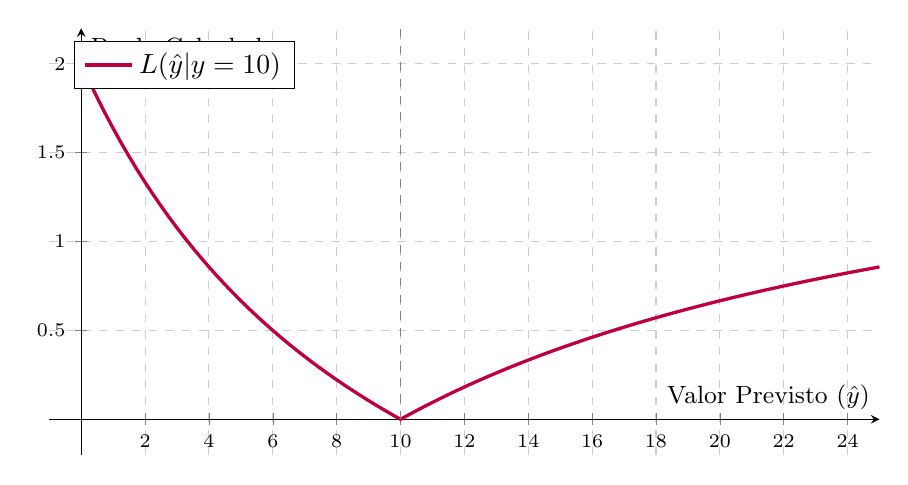
\begin{tikzpicture}
            \begin{axis}[
                % Dimensões ajustadas para caber lado a lado
                width=\linewidth,  
                height=7cm,
                xlabel={Valor Previsto ($\hat{y}$)},
                ylabel={Perda Calculada},
                axis lines=middle,
                grid=major,
                grid style={dashed, gray!40},
                xmin=-1, xmax=25,        % Limites do seu gráfico
                ymin=-0.2, ymax=2.2,         % Limites do seu gráfico
                legend pos=north west,
                title style={font=\bfseries\small},
                label style={font=\small},
                tick label style={font=\scriptsize}
            ]
                % Gráfico da função 2*abs(x - 10) / (abs(x) + 10)
                \addplot[
                    domain=0:25, 
                    samples=101,
                    color=purple, 
                    very thick
                ] {2*abs(x - 10) / (abs(x) + 10)};
                
                \addlegendentry{$L(\hat{y} | y=10)$}

                % Linha vertical para marcar o valor real
                \draw[dashed, gray] (axis cs:10, 0) -- (axis cs:10, 2.2);
                \node[above, gray!80, font=\tiny] at (axis cs:10, 2.2) {Valor Real ($y=10$)};
            \end{axis}
        \end{tikzpicture}
        \caption{Visão 2D (corte em $y=10$).} % Legenda da subfigura
        \label{fig:smape-2d}
    \end{subfigure}
    \hfill % Adiciona espaço horizontal flexível entre as subfiguras
    % --- SUBFIGURA (b): Gráfico 3D da sMAPE ---
    \begin{subfigure}[b]{0.48\textwidth}
        \centering
        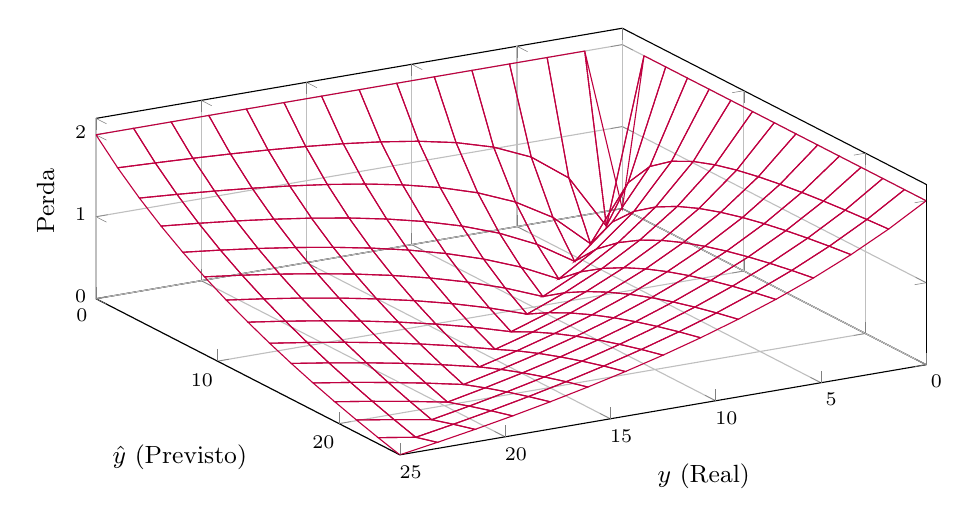
\begin{tikzpicture}
            \begin{axis}[
                % Dimensões consistentes com o gráfico (a)
                width=\linewidth,
                height=7cm,
                xlabel={$y$ (Real)},
                ylabel={$\hat{y}$ (Previsto)},
                zlabel={Perda},
                grid=major,
                view={150}{45}, % Mesmo ângulo de visão do seu template
                zmin=0, zmax=2.2, % sMAPE é limitada entre 0 e 2
                title style={font=\bfseries\small},
                label style={font=\small},
                tick label style={font=\scriptsize}
            ]
                % Gráfico da superfície da sMAPE
                \addplot3[
                    mesh,           
                    color=purple,   % Cor consistente com o gráfico 2D
                    shader=interp,  
                    domain=0:25,    % Domínio de x (y_real)
                    domain y=0:25,  % Domínio de y (y_previsto)
                    samples=15      % Mesma resolução da malha
                ] { 2*abs(x - y) / (abs(x) + abs(y) + 1e-6) }; % L = 2|y - y_hat| / (|y| + |y_hat|)
            \end{axis}
        \end{tikzpicture}
        \caption{Superfície 3D completa.} % Legenda da subfigura
        \label{fig:smape-3d}
    \end{subfigure}

    % --- Legenda e Fonte da Figura Principal ---
    \caption{Visualizações da função de perda sMAPE (\textit{Symmetric Mean Absolute Percentage Error}).}
    \label{fig:smape-loss} % Rótulo principal do seu gráfico
    \fonte{O autor (2025).}
\end{figure}

\medskip
\begin{center}
 * * *
\end{center}
\medskip

\textbf{Características do Erro Percentual Absoluto Médio Simétrico}
\vspace{1em}

\begin{itemize}
    \item \textbf{Característica 1:}
    \item \textbf{Característica 2:}
    \item \textbf{Característica 3:}
\end{itemize}

\medskip
\begin{center}
 * * *
\end{center}
\medskip

\begin{equacaodestaque}{Derivada do Erro Percentual Absoluto Médio Simétrico (\textit{sMAPE})}
    \frac{\partial \Loss_{\text{sMAPE}}}{\partial \hat{y}_j} = \frac{2}{N} \cdot \frac{\text{sgn}(\hat{y}_j - y_j)(\hat{y}_j + y_j) - |\hat{y}_j - y_j|\text{sgn}(\hat{y}_j)}{(\hat{y}_j + y_j)^2}
    \label{eq:smape-derivada}
\end{equacaodestaque}

\begin{figure}[h!]
    \centering % Centraliza a figura na página

    % --- SUBFIGURA (a): Gráfico 2D da Derivada da sMAPE (Corte em y=10) ---
    \begin{subfigure}[b]{0.48\textwidth}
        \centering
        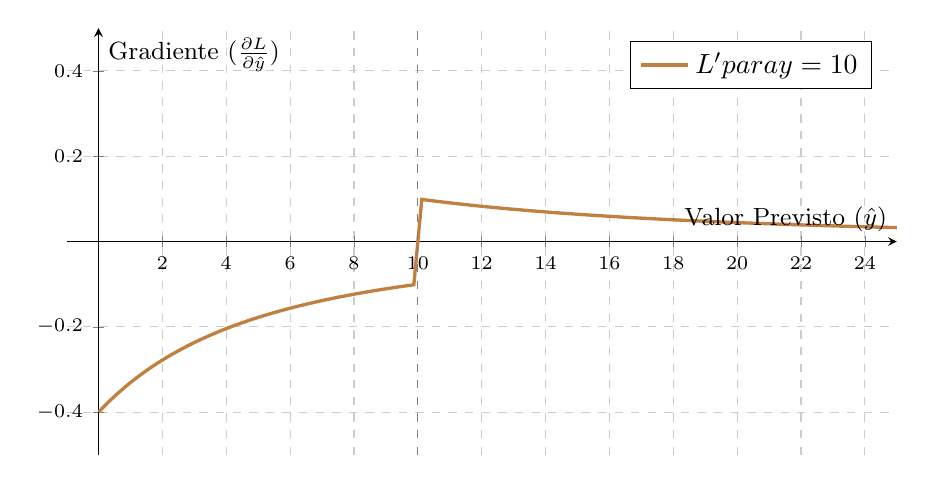
\begin{tikzpicture}
            \begin{axis}[
                % Dimensões ajustadas para caber lado a lado
                width=\linewidth,  
                height=7cm,
                xlabel={Valor Previsto ($\hat{y}$)},
                ylabel={Gradiente ($\frac{\partial L}{\partial \hat{y}}$)},
                axis lines=middle,
                grid=major,
                grid style={dashed, gray!40},
                xmin=-1, xmax=25,        % Limites do seu gráfico
                ymin=-0.5, ymax=0.5,         % Limites do seu gráfico
                legend pos=north east,
                title style={font=\bfseries\small},
                label style={font=\small},
                tick label style={font=\scriptsize},
                declare function={sgn(\x) = (\x > 0) - (\x < 0);} % Função Sinal
            ]
                % Gráfico da derivada
                \addplot[
                    domain=0:25, 
                    samples=201,
                    color=brown, 
                    very thick
                ] {2 * (sgn(x-10)*(x+10) - abs(x-10)) / ((x+10)^2)};
                
                \addlegendentry{$L' \text{ para } y=10$}

                % Linha vertical
                \draw[dashed, gray] (axis cs:10, -0.5) -- (axis cs:10, 0.5);
                \node[above, gray!80, font=\tiny] at (axis cs:10, 0.5) {Valor Real};
            \end{axis}
        \end{tikzpicture}
        \caption{Visão 2D (corte em $y=10$).} % Legenda da subfigura
        \label{fig:smape-derivada-2d}
    \end{subfigure}
    \hfill % Adiciona espaço horizontal flexível entre as subfiguras
    % --- SUBFIGURA (b): Gráfico 3D da Derivada da sMAPE ---
    \begin{subfigure}[b]{0.48\textwidth}
        \centering
        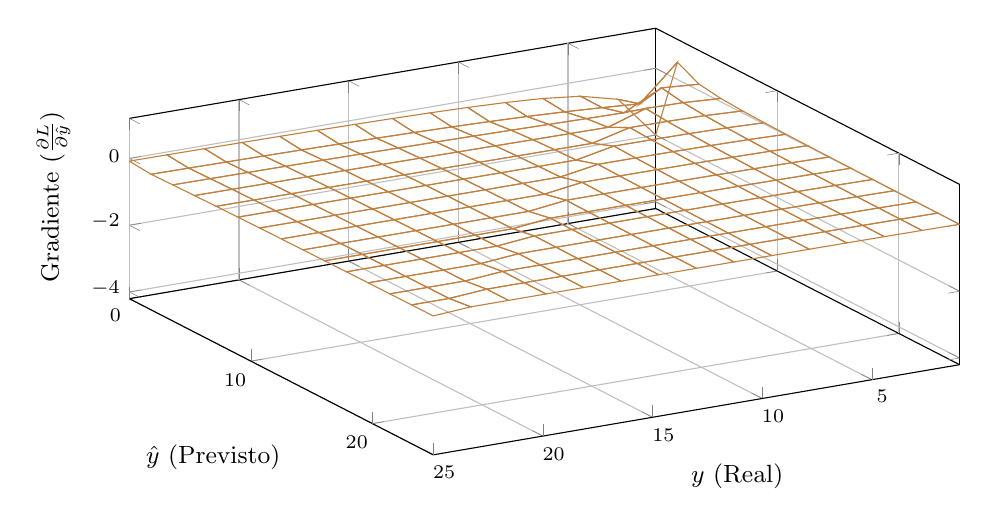
\begin{tikzpicture}
            \begin{axis}[
                % Dimensões consistentes com o gráfico (a)
                width=\linewidth,
                height=7cm,
                xlabel={$y$ (Real)},
                ylabel={$\hat{y}$ (Previsto)},
                zlabel={Gradiente ($\frac{\partial L}{\partial \hat{y}}$)},
                grid=major,
                view={150}{45}, % Mesmo ângulo de visão do seu template
                zmin=-4.2, zmax=1.2, % Gradiente é grande para y pequeno
                title style={font=\bfseries\small},
                label style={font=\small},
                tick label style={font=\scriptsize},
                declare function={sgn(\x) = (\x > 0) - (\x < 0);} % Função Sinal
            ]
                % Gráfico da superfície da derivada da sMAPE
                \addplot3[
                    mesh,           
                    color=brown,    % Cor consistente com o gráfico 2D
                    shader=interp,  
                    domain=1:25,    % Domínio de x (y_real) > 0
                    domain y=0:25,  % Domínio de y (y_previsto)
                    samples=15      % Mesma resolução da malha
                ] { 2 * (sgn(y-x)*(abs(y)+abs(x)) - abs(y-x)*sgn(y)) / ((abs(y)+abs(x))^2) }; % Derivada da sMAPE 3D
            \end{axis}
        \end{tikzpicture}
        \caption{Superfície 3D completa ($y>0$).} % Legenda da subfigura
        \label{fig:smape-derivada-3d}
    \end{subfigure}

    % --- Legenda e Fonte da Figura Principal ---
    \caption{Visualizações da derivada (gradiente) da função de perda sMAPE.}
    \label{fig:smape-derivada} % Rótulo principal do seu gráfico
    \fonte{O autor (2025).}
\end{figure}

\medskip
\begin{center}
 * * *
\end{center}
\medskip

\textbf{Algumas Aplicações do Erro Percentual Absoluto Médio em Problemas de Regressão}
\vspace{1em}

\begin{itemize}
    \item \textbf{Aplicação 1 (Área):}
    \item \textbf{Aplicação 2 (Área):}
    \item \textbf{Aplicação 3 (Área):}
    \item \textbf{Aplicação 4 (Área):}
\end{itemize}

\section{Mudando o Objetivo da Previsão: Além da Média}

\subsection{Perda Quantílica}

\begin{equacaodestaque}{Perda Quantílica (\textit{Quantile Loss})}
    \Loss_{\tau}(y_j, \hat{y}_j) = 
    \begin{cases} 
        \tau (y_j - \hat{y}_j) & \text{se } y_j \ge \hat{y}_j \\
        (1 - \tau)(\hat{y}_j - y_j) & \text{se } y_j < \hat{y}_j
    \end{cases}
    \label{eq:quantile-loss}
\end{equacaodestaque}

\begin{figure}[h!]
    \centering % Centraliza a figura na página

    % --- SUBFIGURA (a): Gráfico 2D da Perda Quantílica ---
    \begin{subfigure}[b]{0.48\textwidth}
        \centering
        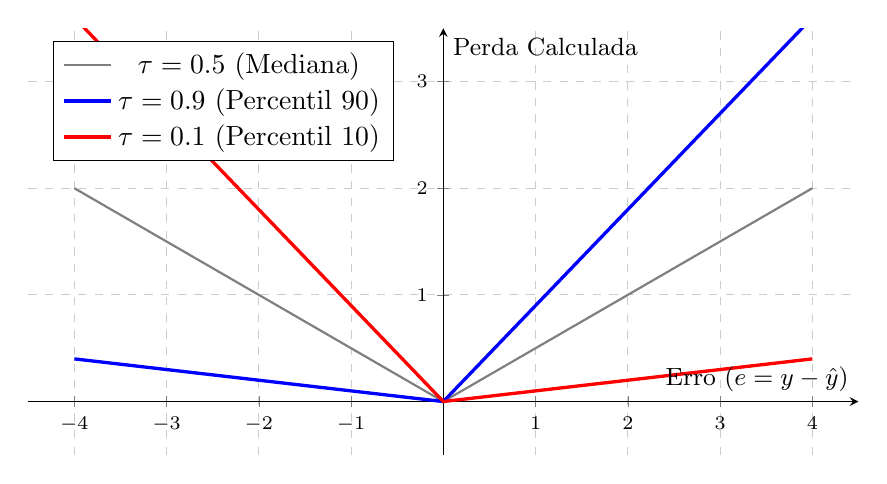
\begin{tikzpicture}
            \begin{axis}[
                % Dimensões ajustadas para caber lado a lado
                width=\linewidth,  
                height=7cm,
                xlabel={Erro ($e = y - \hat{y}$)},
                ylabel={Perda Calculada},
                axis lines=middle,
                grid=major,
                grid style={dashed, gray!40},
                xmin=-4.5, xmax=4.5,        % Limites do seu gráfico
                ymin=-0.5, ymax=3.5,         % Limites do seu gráfico
                legend pos=north west,
                title style={font=\bfseries\small},
                label style={font=\small},
                tick label style={font=\scriptsize}
            ]
                % Tau = 0.5 (MAE)
                \addplot[domain=-4:4, samples=5, color=gray, thick] {0.5*abs(x)};
                \addlegendentry{$\tau=0.5$ (Mediana)}
                
                % Tau = 0.9
                \addplot[domain=-4:4, samples=5, color=blue, very thick] {(x >= 0) ? (0.9*x) : ((1-0.9)*(-x))};
                \addlegendentry{$\tau=0.9$ (Percentil 90)}
                
                % Tau = 0.1
                \addplot[domain=-4:4, samples=5, color=red, very thick] {(x >= 0) ? (0.1*x) : ((1-0.1)*(-x))};
                \addlegendentry{$\tau=0.1$ (Percentil 10)}
            \end{axis}
        \end{tikzpicture}
        \caption{Visão 2D (Perda vs. Erro).} % Legenda da subfigura
        \label{fig:quantile-2d}
    \end{subfigure}
    \hfill % Adiciona espaço horizontal flexível entre as subfiguras
    % --- SUBFIGURA (b): Gráfico 3D da Perda Quantílica ---
    \begin{subfigure}[b]{0.48\textwidth}
        \centering
        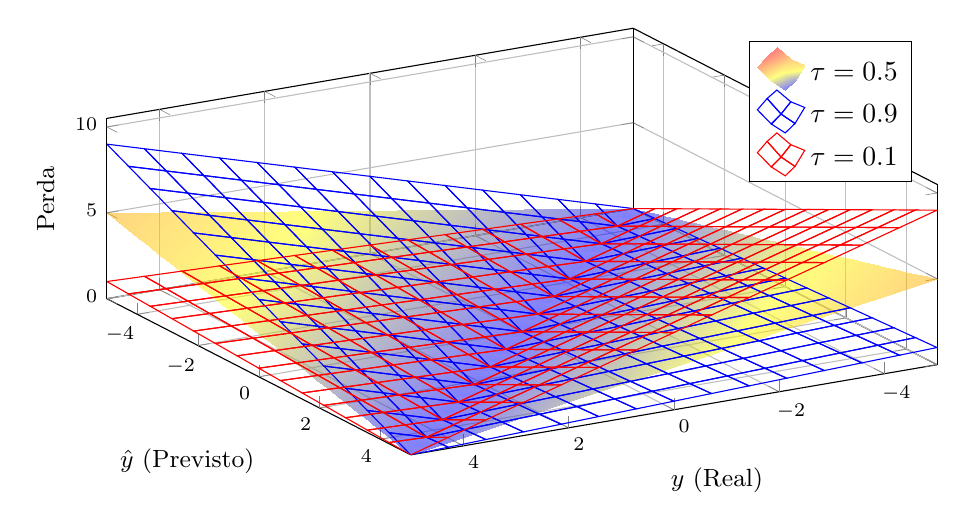
\begin{tikzpicture}
            \begin{axis}[
                % Dimensões consistentes com o gráfico (a)
                width=\linewidth,
                height=7cm,
                xlabel={$y$ (Real)},
                ylabel={$\hat{y}$ (Previsto)},
                zlabel={Perda},
                grid=major,
                view={150}{45}, % Mesmo ângulo de visão do seu template
                zmin=0, zmax=10.5, % Ajustado para o domínio
                legend pos=north east,
                title style={font=\bfseries\small},
                label style={font=\small},
                tick label style={font=\scriptsize}
            ]
                % Tau = 0.5 (Plano de fundo como superfície)
                \addplot3[
                    surf,           % Superfície sólida
                    color=gray,
                    opacity=0.5,    % Semi-transparente
                    shader=interp,
                    domain=-5:5,
                    domain y=-5:5,
                    samples=30      % Mais samples para 'surf' suave
                ] { 0.5*abs(x - y) };
                \addlegendentry{$\tau=0.5$}

                % Tau = 0.9 (Malha)
                \addplot3[
                    mesh,           
                    color=blue,
                    domain=-5:5,
                    domain y=-5:5,
                    samples=15      % Menos samples para 'mesh'
                ] { (x - y >= 0) ? (0.9*(x - y)) : ((1-0.9)*(-(x - y))) };
                \addlegendentry{$\tau=0.9$}
                
                % Tau = 0.1 (Malha)
                \addplot3[
                    mesh,           
                    color=red,
                    domain=-5:5,
                    domain y=-5:5,
                    samples=15
                ] { (x - y >= 0) ? (0.1*(x - y)) : ((1-0.1)*(-(x - y))) };
                \addlegendentry{$\tau=0.1$}
            \end{axis}
        \end{tikzpicture}
        \caption{Superfície 3D completa.} % Legenda da subfigura
        \label{fig:quantile-3d}
    \end{subfigure}

    % --- Legenda e Fonte da Figura Principal ---
    \caption{Visualizações da Perda Quantílica (\textit{Pinball Loss}) em duas e em três dimensões.}
    \label{fig:quantile-loss} % Rótulo principal do seu gráfico
    \fonte{O autor (2025).}
\end{figure}

\medskip
\begin{center}
 * * *
\end{center}
\medskip

\textbf{Características da Perda Quantílica}
\vspace{1em}

\begin{itemize}
    \item \textbf{Característica 1:}
    \item \textbf{Característica 2:}
    \item \textbf{Característica 3:}
\end{itemize}

\medskip
\begin{center}
 * * *
\end{center}
\medskip

\begin{equacaodestaque}{Derivada da Perda Quantílica}
    \frac{\partial \Loss_{\tau}}{\partial \hat{y}_j} = 
    \begin{cases} 
        -(1 - \tau) & \text{se } y_j < \hat{y}_j \text{ (superestimação)}\\
        -\tau & \text{se } y_j > \hat{y}_j \text{ (subestimação)}
    \end{cases}
    \label{eq:quantile-loss-derivada}
\end{equacaodestaque}

\begin{figure}[h!]
    \centering
    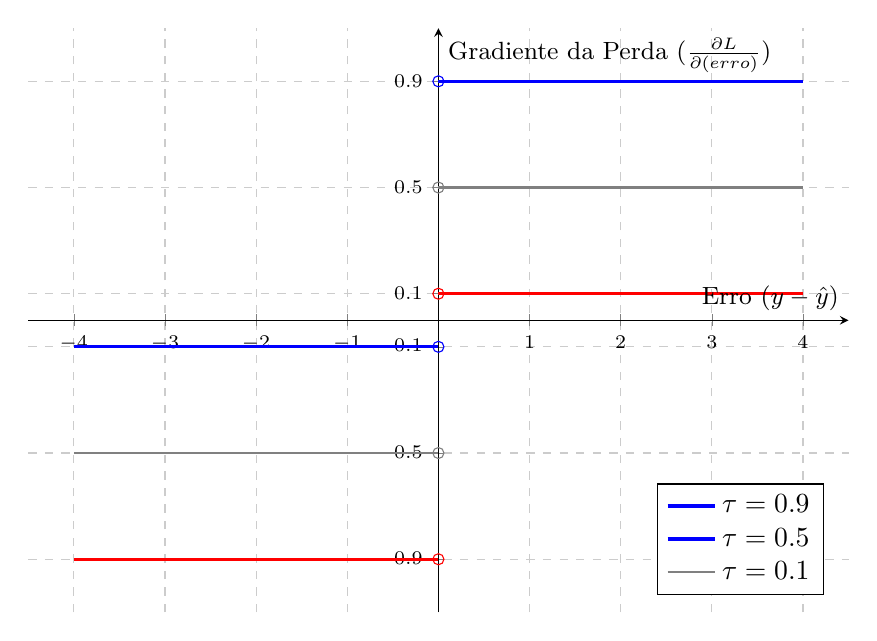
\begin{tikzpicture}
        \begin{axis}[
            xlabel={Erro ($y - \hat{y}$)},
            ylabel={Gradiente da Perda ($\frac{\partial L}{\partial (\text{erro})}$)},
            axis lines=middle,
            grid=major,
            grid style={dashed, gray!40},
            xmin=-4.5, xmax=4.5,
            ymin=-1.1, ymax=1.1,
            ytick={-0.9, -0.5, -0.1, 0, 0.1, 0.5, 0.9},
            legend pos=south east,
            width=12cm,
            height=9cm,
            title style={font=\bfseries},
            label style={font=\small},
            tick label style={font=\scriptsize}
        ]
            % Linhas para Tau = 0.9
            \addplot[const plot, color=blue, very thick] coordinates {(-4, 0.9-1) (0, 0.9-1)};
            \addplot[const plot, color=blue, very thick] coordinates {(0, 0.9) (4, 0.9)};
            \addlegendentry{$\tau=0.9$}
            
            % Linhas para Tau = 0.5
            \addplot[const plot, color=gray, thick] coordinates {(-4, 0.5-1) (0, 0.5-1)};
            \addplot[const plot, color=gray, thick] coordinates {(0, 0.5) (4, 0.5)};
            \addlegendentry{$\tau=0.5$}

            % Linhas para Tau = 0.1
            \addplot[const plot, color=red, very thick] coordinates {(-4, 0.1-1) (0, 0.1-1)};
            \addplot[const plot, color=red, very thick] coordinates {(0, 0.1) (4, 0.1)};
            \addlegendentry{$\tau=0.1$}

            % Círculos abertos para a descontinuidade
            \addplot[only marks, mark=o, color=blue, mark size=2pt] coordinates {(0, -0.1) (0, 0.9)};
            \addplot[only marks, mark=o, color=gray, mark size=2pt] coordinates {(0, -0.5) (0, 0.5)};
            \addplot[only marks, mark=o, color=red, mark size=2pt] coordinates {(0, -0.9) (0, 0.1)};
        \end{axis}
    \end{tikzpicture}
    \caption{Gráfico da derivada da Perda Quantílica (em relação ao erro). O gradiente é uma função de degrau assimétrica.}
    \label{fig:quantile-loss-derivada}
    \fonte{O autor (2025).}
\end{figure}

\medskip
\begin{center}
 * * *
\end{center}
\medskip

\textbf{Algumas Aplicações da Perda Quantília em Problemas de Regressão}
\vspace{1em}

\begin{itemize}
    \item \textbf{Aplicação 1 (Área):}
    \item \textbf{Aplicação 2 (Área):}
    \item \textbf{Aplicação 3 (Área):}
    \item \textbf{Aplicação 4 (Área):}
\end{itemize}

\subsection{Perda Epsilon-Insensível}

\begin{equacaodestaque}{Perda Epsilon-Insensível (\textit{$\epsilon$-Insensitive Loss})}
    \Loss_{\epsilon}(y, \hat{y}) = 
    \begin{cases} 
        0 & \text{se } |y - \hat{y}| \le \epsilon \\
        |y - \hat{y}| - \epsilon & \text{se } |y - \hat{y}| > \epsilon
    \end{cases}
    \label{eq:epsilon-insensitive-loss}
\end{equacaodestaque}

\begin{figure}[h!]
    \centering % Centraliza a figura na página

    % --- SUBFIGURA (a): Gráfico 2D da Epsilon-Insensitive Loss ---
    \begin{subfigure}[b]{0.48\textwidth}
        \centering
        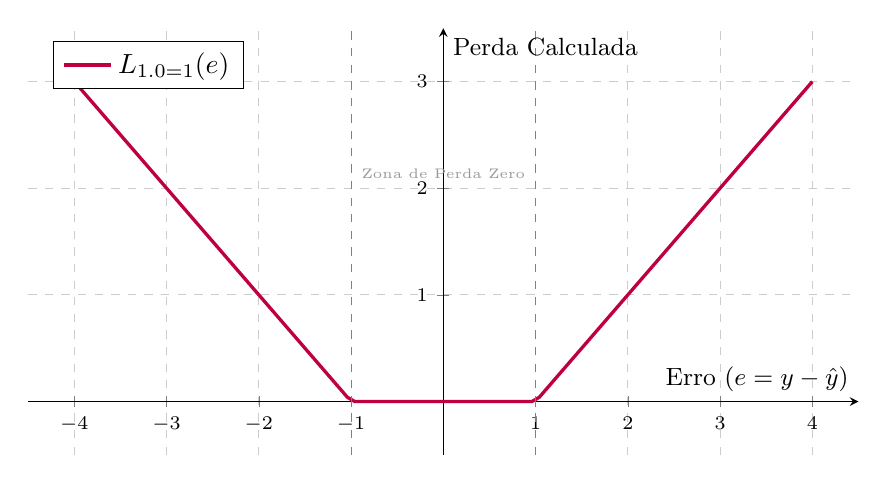
\begin{tikzpicture}
            % Define o valor de epsilon
            \def\epsilon{1.0}
            
            \begin{axis}[
                % Dimensões ajustadas para caber lado a lado
                width=\linewidth,  
                height=7cm,
                xlabel={Erro ($e = y - \hat{y}$)},
                ylabel={Perda Calculada},
                axis lines=middle,
                grid=major,
                grid style={dashed, gray!40},
                xmin=-4.5, xmax=4.5,        % Limites do seu gráfico
                ymin=-0.5, ymax=3.5,         % Limites do seu gráfico
                legend pos=north west,
                title style={font=\bfseries\small},
                label style={font=\small},
                tick label style={font=\scriptsize}
            ]
                % Gráfico da função
                \addplot[
                    domain=-4:4, 
                    samples=101,
                    color=purple, 
                    very thick
                ] {max(0, abs(x) - \epsilon)};
                
                \addlegendentry{$L_{\epsilon=1}(e)$}

                % Linhas tracejadas para marcar a margem epsilon
                \draw[dashed, gray] (axis cs:-\epsilon, -0.5) -- (axis cs:-\epsilon, 3.5);
                \draw[dashed, gray] (axis cs:\epsilon, -0.5) -- (axis cs:\epsilon, 3.5);
                \node[above, gray!80, font=\tiny] at (axis cs:0, 2) {Zona de Perda Zero};
            \end{axis}
        \end{tikzpicture}
        \caption{Visão 2D (Perda vs. Erro).} % Legenda da subfigura
        \label{fig:epsilon-2d}
    \end{subfigure}
    \hfill % Adiciona espaço horizontal flexível entre as subfiguras
    % --- SUBFIGURA (b): Gráfico 3D da Epsilon-Insensitive Loss ---
    \begin{subfigure}[b]{0.48\textwidth}
        \centering
        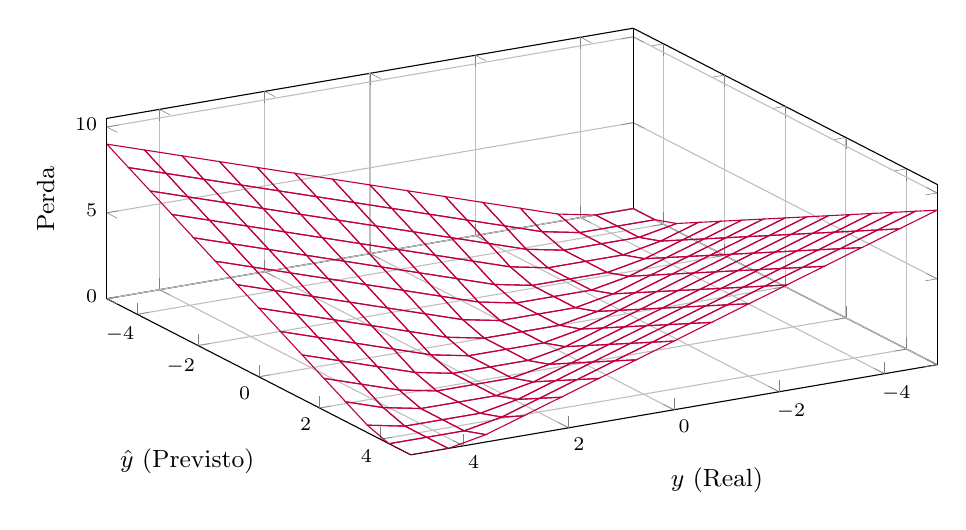
\begin{tikzpicture}
            % Define o valor de epsilon
            \def\epsilon{1.0}
            
            \begin{axis}[
                % Dimensões consistentes com o gráfico (a)
                width=\linewidth,
                height=7cm,
                xlabel={$y$ (Real)},
                ylabel={$\hat{y}$ (Previsto)},
                zlabel={Perda},
                grid=major,
                view={150}{45}, % Mesmo ângulo de visão do seu template
                zmin=0, zmax=10.5, % Ajustado para max(0, abs(10) - 1) = 9
                title style={font=\bfseries\small},
                label style={font=\small},
                tick label style={font=\scriptsize}
            ]
                % Gráfico da superfície da Epsilon-Insensitive Loss
                \addplot3[
                    mesh,           
                    color=purple,   % Cor consistente com o gráfico 2D
                    shader=interp,  
                    domain=-5:5,    % Mesmo domínio do seu template
                    domain y=-5:5,  % Mesmo domínio do seu template
                    samples=15      % Mesma resolução da malha
                ] { max(0, abs(x - y) - \epsilon) }; % A função Epsilon-Insensitive 3D
            \end{axis}
        \end{tikzpicture}
        \caption{Superfície 3D completa.} % Legenda da subfigura
        \label{fig:epsilon-3d}
    \end{subfigure}

    % --- Legenda e Fonte da Figura Principal ---
    \caption{Visualizações da função de perda Epsilon-Insensível (\textit{Epsilon-Insensitive Loss}, $\epsilon=1$) em duas e em três dimensões.}
    \label{fig:epsilon-insensitive-loss} % Rótulo principal do seu gráfico
    \fonte{O autor (2025).}
\end{figure}

\medskip
\begin{center}
 * * *
\end{center}
\medskip

\textbf{Características da Perda Epsilon-Insensível}
\vspace{1em}

\begin{itemize}
    \item \textbf{Característica 1:}
    \item \textbf{Característica 2:}
    \item \textbf{Característica 3:}
\end{itemize}

\medskip
\begin{center}
 * * *
\end{center}
\medskip

\begin{equacaodestaque}{Derivada da Perda Epsilon-Insensível}
    \frac{\partial \Loss_{\epsilon}}{\partial \hat{y}} = 
    \begin{cases} 
        -1 & \text{se } \hat{y} - y > \epsilon \\
        0 & \text{se } |\hat{y} - y| \le \epsilon \\
        1 & \text{se } \hat{y} - y < -\epsilon
    \end{cases}
    \label{eq:epsilon-insensitive-derivada}
\end{equacaodestaque}

\begin{figure}[h!]
    \centering
    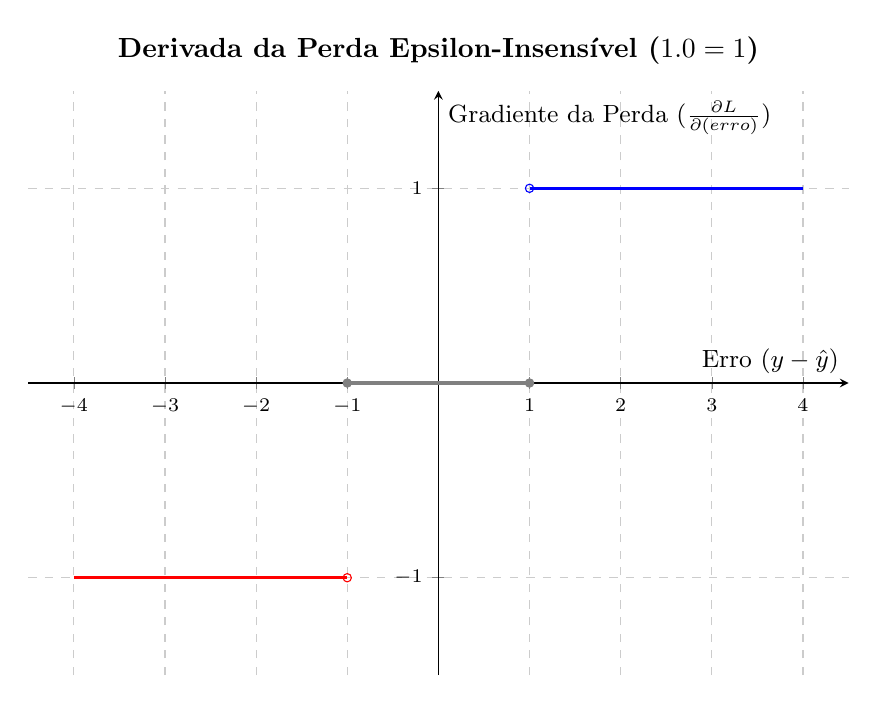
\begin{tikzpicture}
        \begin{axis}[
            title={Derivada da Perda Epsilon-Insensível ($\epsilon=1$)},
            xlabel={Erro ($y - \hat{y}$)},
            ylabel={Gradiente da Perda ($\frac{\partial L}{\partial (\text{erro})}$)},
            axis lines=middle,
            grid=major,
            grid style={dashed, gray!40},
            xmin=-4.5, xmax=4.5,
            ymin=-1.5, ymax=1.5,
            ytick={-1, 0, 1},
            legend pos=north west,
            width=12cm,
            height=9cm,
            title style={font=\bfseries},
            label style={font=\small},
            tick label style={font=\scriptsize}
        ]
            % Define o valor de epsilon
            \def\epsilon{1.0}

            % Parte negativa da derivada (-1)
            \addplot[const plot, color=red, very thick] coordinates {(-4, -1) (-\epsilon, -1)};
            
            % Parte central da derivada (0)
            \addplot[const plot, color=gray, very thick] coordinates {(-\epsilon, 0) (\epsilon, 0)};
            
            % Parte positiva da derivada (+1)
            \addplot[const plot, color=blue, very thick] coordinates {(\epsilon, 1) (4, 1)};
            
            % Círculos abertos/fechados para as descontinuidades
            \addplot[only marks, mark=*, color=gray, mark size=1.5pt] coordinates {(-\epsilon, 0) (\epsilon, 0)};
            \addplot[only marks, mark=o, color=red, mark size=1.5pt] coordinates {(-\epsilon, -1)};
            \addplot[only marks, mark=o, color=blue, mark size=1.5pt] coordinates {(\epsilon, 1)};
            
        \end{axis}
    \end{tikzpicture}
    \caption{Gráfico da derivada da Perda Epsilon-Insensível. O gradiente é zero dentro da margem $\epsilon$.}
    \label{fig:epsilon-insensitive-derivada}
    \fonte{O autor (2025).}
\end{figure}

\medskip
\begin{center}
 * * *
\end{center}
\medskip

\textbf{Algumas Aplicações da Perda Epsilon-Insensível em Problemas de Regressão}
\vspace{1em}

\begin{itemize}
    \item \textbf{Aplicação 1 (Área):}
    \item \textbf{Aplicação 2 (Área):}
    \item \textbf{Aplicação 3 (Área):}
    \item \textbf{Aplicação 4 (Área):}
\end{itemize}

\section{Perdas Baseadas em Distribuições de Dados}

\subsection{Perda de Poisson}

\begin{equacaodestaque}{Perda de Poisson (\textit{Poisson Loss})}
    \Loss_{\text{Poisson}}(y_j, \hat{y}_j) = \hat{y}_j - y_j \log(\hat{y}_j)
    \label{eq:poisson-loss}
\end{equacaodestaque}

\begin{figure}[h!]
    \centering
    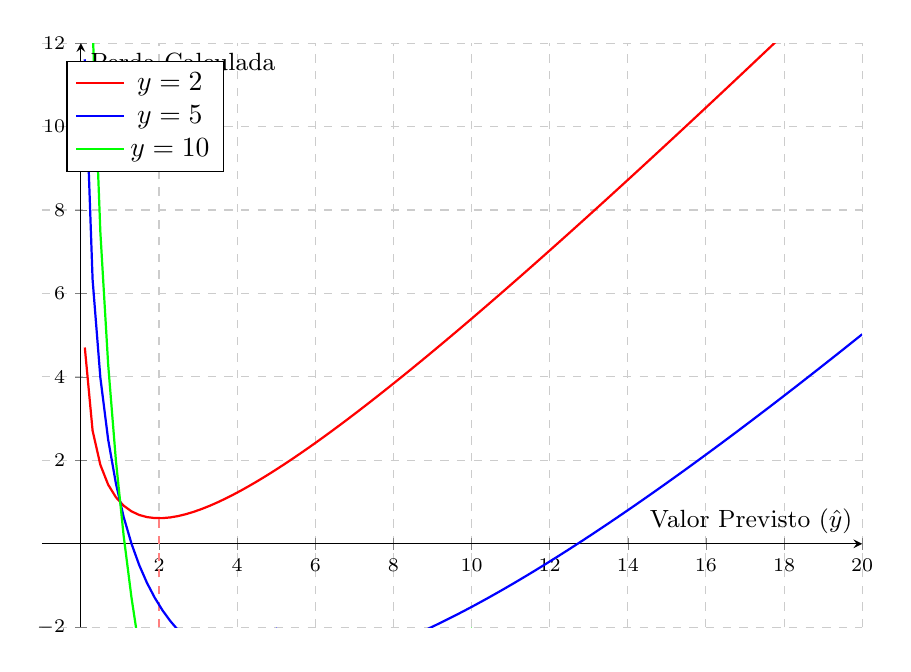
\begin{tikzpicture}
        \begin{axis}[
            xlabel={Valor Previsto ($\hat{y}$)},
            ylabel={Perda Calculada},
            axis lines=middle,
            grid=major,
            grid style={dashed, gray!40},
            xmin=-1, xmax=20,
            ymin=-2, ymax=12,
            legend pos=north west,
            width=12cm,
            height=9cm,
            title style={font=\bfseries},
            label style={font=\small},
            tick label style={font=\scriptsize}
        ]
            % Curva para y=2
            \addplot[domain=0.1:20, samples=101, color=red, thick] {x - 2*ln(x)};
            \addlegendentry{$y=2$}
            \draw[dashed, red!50] (axis cs:2, -2) -- (axis cs:2, {2-2*ln(2)});

            % Curva para y=5
            \addplot[domain=0.1:20, samples=101, color=blue, thick] {x - 5*ln(x)};
            \addlegendentry{$y=5$}
            \draw[dashed, blue!50] (axis cs:5, -2) -- (axis cs:5, {5-5*ln(5)});

            % Curva para y=10
            \addplot[domain=0.1:20, samples=101, color=green, thick] {x - 10*ln(x)};
            \addlegendentry{$y=10$}
            \draw[dashed, green!50] (axis cs:10, -2) -- (axis cs:10, {10-10*ln(10)});
            
        \end{axis}
    \end{tikzpicture}
    \caption{Gráfico da Perda de Poisson para diferentes valores reais de $y$. O mínimo de cada curva ocorre em $\hat{y}=y$.}
    \label{fig:poisson-loss}
    \fonte{O autor (2025).}
\end{figure}

\medskip
\begin{center}
 * * *
\end{center}
\medskip

\textbf{Características da Perda de Poisson}
\vspace{1em}

\begin{itemize}
    \item \textbf{Característica 1:}
    \item \textbf{Característica 2:}
    \item \textbf{Característica 3:}
\end{itemize}

\medskip
\begin{center}
 * * *
\end{center}
\medskip

\begin{equacaodestaque}{Derivada da Perda de Poisson}
    \frac{\partial \Loss_{\text{Poisson}}}{\partial \hat{y}_j} = 1 - \frac{y_j}{\hat{y}_j} = \frac{\hat{y}_j - y_j}{\hat{y}_j}
    \label{eq:poisson-loss-derivada}
\end{equacaodestaque}

\begin{figure}[h!]
    \centering
    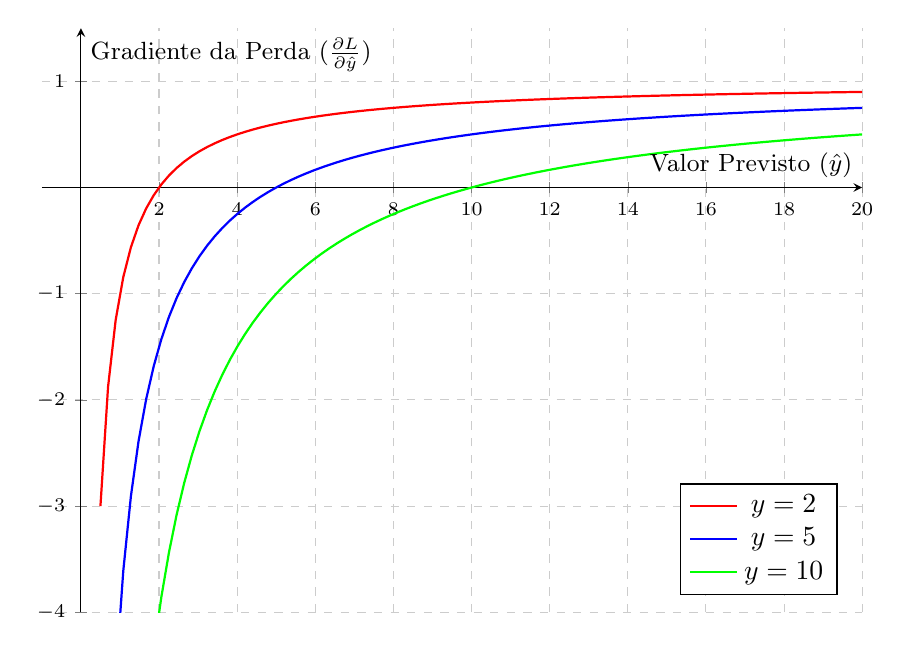
\begin{tikzpicture}
        \begin{axis}[
            xlabel={Valor Previsto ($\hat{y}$)},
            ylabel={Gradiente da Perda ($\frac{\partial L}{\partial \hat{y}}$)},
            axis lines=middle,
            grid=major,
            grid style={dashed, gray!40},
            xmin=-1, xmax=20,
            ymin=-4, ymax=1.5,
            legend pos=south east,
            width=12cm,
            height=9cm,
            title style={font=\bfseries},
            label style={font=\small},
            tick label style={font=\scriptsize}
        ]
            % Curva para y=2
            \addplot[domain=0.5:20, samples=101, color=red, thick] {1 - 2/x};
            \addlegendentry{$y=2$}
            
            % Curva para y=5
            \addplot[domain=0.5:20, samples=101, color=blue, thick] {1 - 5/x};
            \addlegendentry{$y=5$}

            % Curva para y=10
            \addplot[domain=0.5:20, samples=101, color=green, thick] {1 - 10/x};
            \addlegendentry{$y=10$}
            
        \end{axis}
    \end{tikzpicture}
    \caption{Gráfico da derivada da Perda de Poisson. O gradiente é zero quando $\hat{y}=y$ e assintótico a 1 para $\hat{y} \to \infty$.}
    \label{fig:poisson-loss-derivada}
    \fonte{O autor (2025).}
\end{figure}

\medskip
\begin{center}
 * * *
\end{center}
\medskip

\textbf{Algumas Aplicações da Perda de Poisson em Problemas de Regressão}
\vspace{1em}

\begin{itemize}
    \item \textbf{Aplicação 1 (Área):}
    \item \textbf{Aplicação 2 (Área):}
    \item \textbf{Aplicação 3 (Área):}
    \item \textbf{Aplicação 4 (Área):}
\end{itemize}

\subsection{Perda de Tweedie}

\begin{equacaodestaque}{Perda de Tweedie (\textit{Tweedie Loss})}
    \Loss_{\text{Tweedie}}(y_j, \hat{y}_j; p) = -\frac{y_j \cdot \hat{y}_j^{1-p}}{1-p} + \frac{\hat{y}_j^{2-p}}{2-p}
    \label{eq:tweedie-loss}
\end{equacaodestaque}

\begin{figure}[h!]
    \centering
    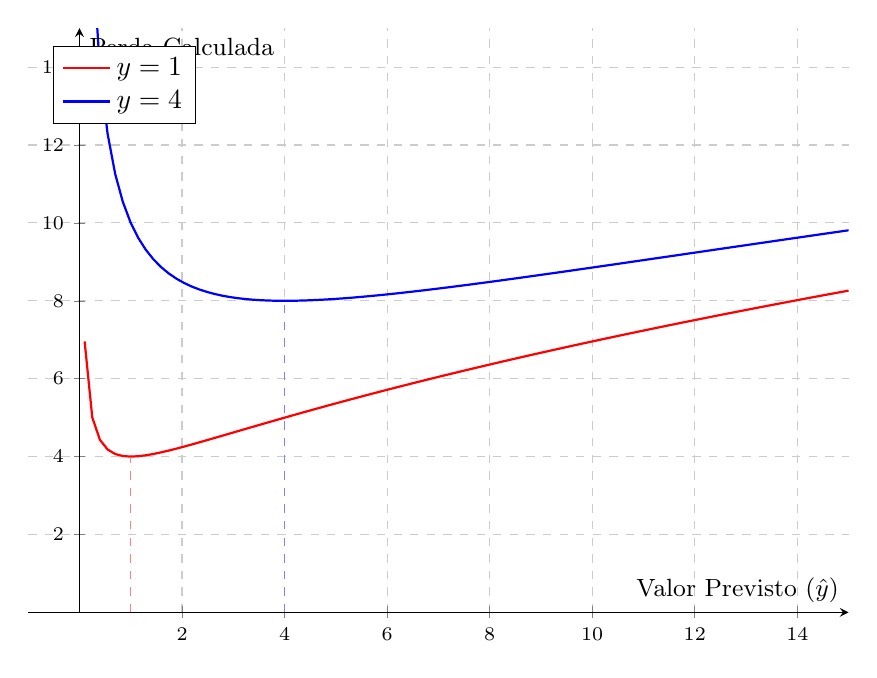
\begin{tikzpicture}
        \begin{axis}[
            xlabel={Valor Previsto ($\hat{y}$)},
            ylabel={Perda Calculada},
            axis lines=middle,
            grid=major,
            grid style={dashed, gray!40},
            xmin=-1, xmax=15,
            ymin=0, ymax=15,
            legend pos=north west,
            width=12cm,
            height=9cm,
            title style={font=\bfseries},
            label style={font=\small},
            tick label style={font=\scriptsize}
        ]
            % Definição do parâmetro p
            \def\p{1.5}

            % Curva para y=1
            \addplot[domain=0.1:15, samples=101, color=red, thick] 
                { -1*x^(1-\p)/(1-\p) + x^(2-\p)/(2-\p) };
            \addlegendentry{$y=1$}
            \draw[dashed, red!50] (axis cs:1, 0) -- (axis cs:1, {-1*1^(1-\p)/(1-\p) + 1^(2-\p)/(2-\p)});

            % Curva para y=4
            \addplot[domain=0.1:15, samples=101, color=blue, thick] 
                { -4*x^(1-\p)/(1-\p) + x^(2-\p)/(2-\p) };
            \addlegendentry{$y=4$}
            \draw[dashed, blue!50] (axis cs:4, 0) -- (axis cs:4, {-4*4^(1-\p)/(1-\p) + 4^(2-\p)/(2-\p)});
            
        \end{axis}
    \end{tikzpicture}
    \caption{Gráfico da Perda de Tweedie para $p=1.5$. O mínimo de cada curva ocorre em $\hat{y}=y$.}
    \label{fig:tweedie-loss}
    \fonte{O autor (2025).}
\end{figure}

\medskip
\begin{center}
 * * *
\end{center}
\medskip

\textbf{Características da Perda de Tweedie}
\vspace{1em}

\begin{itemize}
    \item \textbf{Característica 1:}
    \item \textbf{Característica 2:}
    \item \textbf{Característica 3:}
\end{itemize}

\medskip
\begin{center}
 * * *
\end{center}
\medskip

\begin{equacaodestaque}{Derivada da Perda de Tweedie}
    \frac{\partial \Loss_{\text{Tweedie}}}{\partial \hat{y}_j} = \hat{y}_j^{-p}(\hat{y}_j - y_j)
    \label{eq:tweedie-loss-derivada}
\end{equacaodestaque}

\begin{figure}[h!]
    \centering
    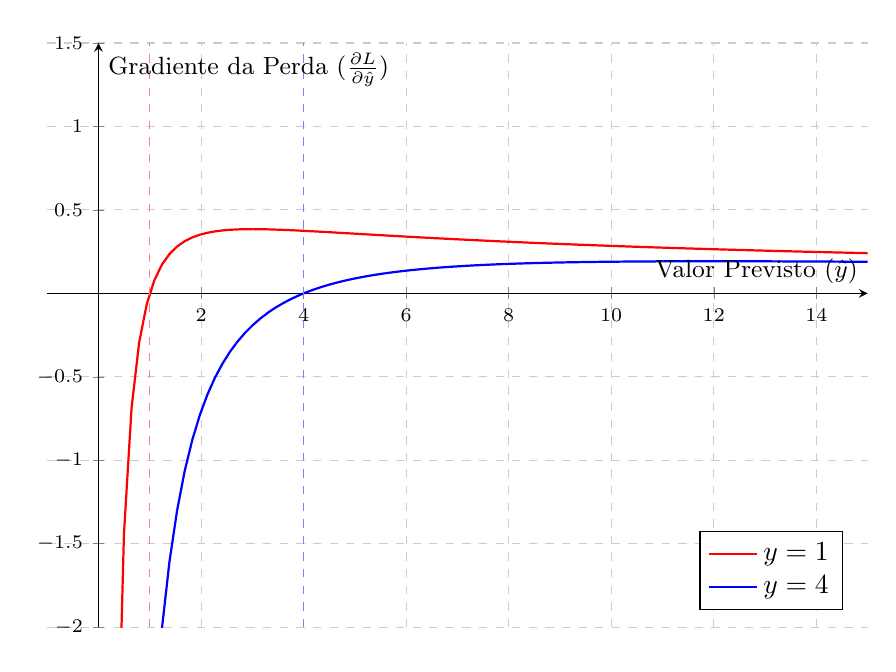
\begin{tikzpicture}
        \begin{axis}[
            xlabel={Valor Previsto ($\hat{y}$)},
            ylabel={Gradiente da Perda ($\frac{\partial L}{\partial \hat{y}}$)},
            axis lines=middle,
            grid=major,
            grid style={dashed, gray!40},
            xmin=-1, xmax=15,
            ymin=-2, ymax=1.5,
            legend pos=south east,
            width=12cm,
            height=9cm,
            title style={font=\bfseries},
            label style={font=\small},
            tick label style={font=\scriptsize}
        ]
            % Definição do parâmetro p
            \def\p{1.5}
            
            % Curva para y=1
            \addplot[domain=0.2:15, samples=101, color=red, thick] 
                {x^(-\p)*(x-1)};
            \addlegendentry{$y=1$}
            
            % Curva para y=4
            \addplot[domain=0.2:15, samples=101, color=blue, thick] 
                {x^(-\p)*(x-4)};
            \addlegendentry{$y=4$}

            % Linhas verticais onde o gradiente é zero
            \draw[dashed, red!50] (axis cs:1, -2) -- (axis cs:1, 1.5);
            \draw[dashed, blue!50] (axis cs:4, -2) -- (axis cs:4, 1.5);
            
        \end{axis}
    \end{tikzpicture}
    \caption{Gráfico da derivada da Perda de Tweedie para $p=1.5$. O gradiente é zero quando a previsão é igual ao valor real.}
    \label{fig:tweedie-loss-derivada}
    \fonte{O autor (2025).}
\end{figure}

\medskip
\begin{center}
 * * *
\end{center}
\medskip

\textbf{Algumas Aplicações da Perda de Tweedie}
\vspace{1em}

\begin{itemize}
    \item \textbf{Aplicação 1 (Área):}
    \item \textbf{Aplicação 2 (Área):}
    \item \textbf{Aplicação 3 (Área):}
    \item \textbf{Aplicação 4 (Área):}
\end{itemize}

\subsection{Divergência Kullback-Leibler}

\begin{equacaodestaque}{Divergência KL entre duas Gaussianas}
    D_{KL}(P || Q) = \log\frac{\sigma_2}{\sigma_1} + \frac{\sigma_1^2 + (\mu_1 - \mu_2)^2}{2\sigma_2^2} - \frac{1}{2}
    \label{eq:kl-divergence-gaussiana}
\end{equacaodestaque}

\begin{figure}[h!]
    \centering
    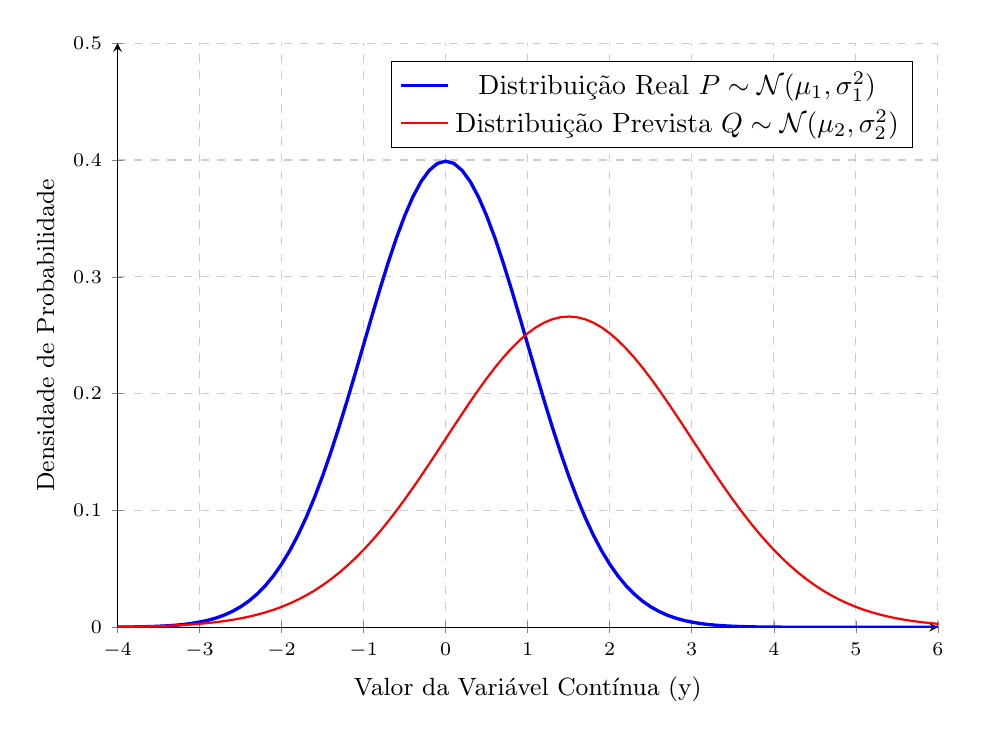
\begin{tikzpicture}
        \begin{axis}[
            xlabel={Valor da Variável Contínua (y)},
            ylabel={Densidade de Probabilidade},
            axis lines=left,
            grid=major,
            grid style={dashed, gray!40},
            xmin=-4, xmax=6,
            ymin=0, ymax=0.5,
            legend pos=north east,
            width=12cm,
            height=9cm,
            title style={font=\bfseries},
            label style={font=\small},
            tick label style={font=\scriptsize}
        ]
            % Distribuição Real P
            \addplot[
                domain=-4:6, samples=101, color=blue, very thick,
                ] {exp(-(x-0)^2 / (2*1^2)) / (1 * sqrt(2*pi))};
            \addlegendentry{Distribuição Real $P \sim \mathcal{N}(\mu_1, \sigma_1^2)$}

            % Distribuição Prevista Q
            \addplot[
                domain=-4:6, samples=101, color=red, thick,
            ] {exp(-(x-1.5)^2 / (2*1.5^2)) / (1.5 * sqrt(2*pi))};
            \addlegendentry{Distribuição Prevista $Q \sim \mathcal{N}(\mu_2, \sigma_2^2)$}
            
        \end{axis}
    \end{tikzpicture}
    \caption{A Divergência KL mede a diferença entre a distribuição prevista pelo modelo ($Q$) e a distribuição real dos dados ($P$).}
    \label{fig:kl-divergence-concept-regressao}
    \fonte{O autor (2025).}
\end{figure}

\medskip
\begin{center}
 * * *
\end{center}
\medskip

\textbf{Características da Divergência de Kullback-Leibler}
\vspace{1em}

\begin{itemize}
    \item \textbf{Característica 1:}
    \item \textbf{Característica 2:}
    \item \textbf{Característica 3:}
\end{itemize}

\medskip
\begin{center}
 * * *
\end{center}
\medskip

\begin{equacaodestaque}{Derivadas da Divergência KL (Gaussiana)}
    \frac{\partial D_{KL}}{\partial \mu_2} = \frac{\mu_2 - \mu_1}{\sigma_2^2}
    \\[10pt] % Espaçamento vertical
    \frac{\partial D_{KL}}{\partial \sigma_2} = \frac{1}{\sigma_2} - \frac{\sigma_1^2 + (\mu_1 - \mu_2)^2}{\sigma_2^3}
    \label{eq:kl-divergence-derivada-gaussiana}
\end{equacaodestaque}

\medskip
\begin{center}
 * * *
\end{center}
\medskip

\textbf{Algumas Aplicações da Divergência de Kullback-Leibler em Problemas de Regressão}
\vspace{1em}

\begin{itemize}
    \item \textbf{Aplicação 1 (Área):}
    \item \textbf{Aplicação 2 (Área):}
    \item \textbf{Aplicação 3 (Área):}
    \item \textbf{Aplicação 4 (Área):}
\end{itemize}

\section{Comparativo: Funções de Perda para Regressão}

\section{Fluxograma: Escolhendo a Função de Perda Ideal}
